
\chapter{Analysis of Protein \npistar{} Interactions}

\begin{quote}
{\it
  Whether you can observe a thing or not depends on the theory which you use.
  It is the theory which decides what can be observed.}
\\\\
 -- Albert Einstein
\end{quote}

\section{Introduction}

\begin{doublespace}
Proteins exhibit a diversity of structures, with 2,738 folds or topologies
present in the CATH database \cite{knudsen:hugen2010}. Each unique
structure is defined by its amino acid composition, where sequence identities
greater than 40\% imply homologous structures \cite{rost:proteng1999}.
Predicting the three-dimensional conformation of a protein from its primary
sequence is a fundamental challenge of structural biology, and achieving this
goal requires a thorough understanding of the underlying interactions and
forces that stabilize protein structures \cite{zhang:opin2008}.
\\\\
Hydrophobic interactions and hydrogen bonds are two of the most common forces
attributed to the overall stability of protein structures
\cite{robertson:chemrev1997,dill:bioc1990}. The burial of hydrophobic
residues is generally considered a major driving force in protein folding
\cite{kauzmann:apc1959} and has been predicted to contribute roughly
8 kJ/mol per buried residue. Conversely, the contribution of hydrogen bonds to
protein structure stability has been controversial
\cite{pace:nsmb2009}. Hydrogen bonds have been described as
destabilizing, partially stabilizing or important driving forces. Of course,
hydrogen bonds are a defining feature of $\alpha$-helices, $\beta$-sheets and
turns. Thus, the generally accepted view is that hydrogen bonds within a
protein structure are marginally favored over hydrogen bonds to water.
Hydrogen bonds are estimated to contribute roughly 4 kJ/mol to protein
stability, but can vary based on the polarity of the microenvironment
\cite{gao:nsmb2009}. Despite these observations, a satisfying
general mechanism for protein folding has not yet been described
\cite{shakhnovich:pnas2009,shaw:sci2010}, which strongly implies
that our understanding of the factors involved in protein folding and stability
is incomplete.
\end{doublespace}

\begin{figure}[ht!]
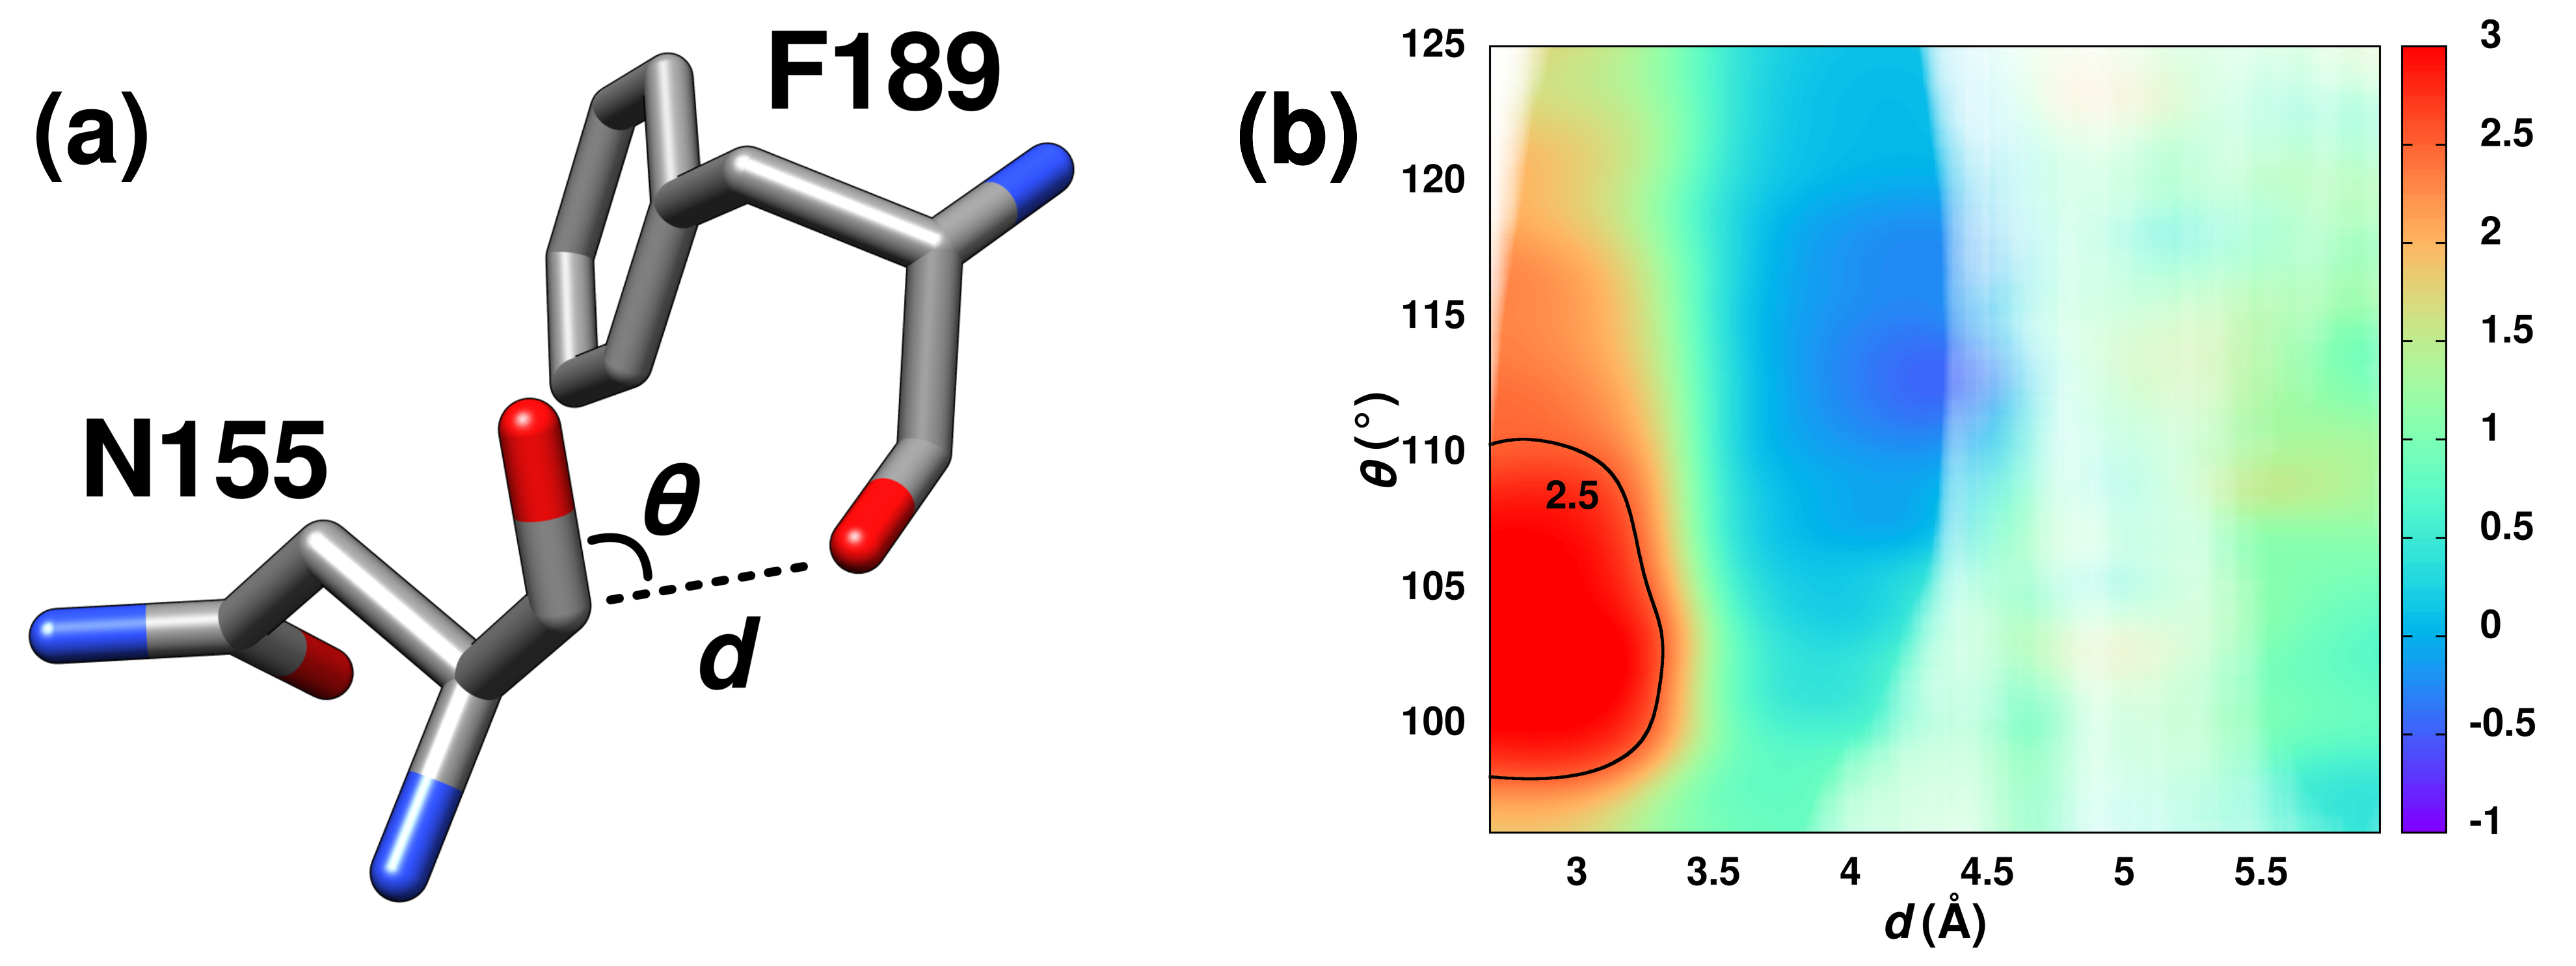
\includegraphics[width=6.5in]{figs/npistar/01.png}
\caption
      [Predicted \npistar{} Interaction and Associated Carbonyl \cnmr{}
       Chemical Shifts.]{
  {\bf Predicted \npistar{} Interaction and Associated Carbonyl \cnmr{}
       Chemical Shifts.
  }
  \\
  ({\bf A}) Residues Asn155 and Phe189 from the x-ray structure of
  \emph{Bacillus amyloliquefaciens} subtillisin BPN' (PDB ID: 1v5i)
  illustrating the structural features for an optimal \npistar{} interaction
  between carbonyl groups.
  ({\bf B}) 2D contour plot of carbonyl \cnmr{} chemical shift differences
  relative to random coil values as a function of the distance ($d$) and
  angle ($\theta$) between carbonyls. A Gaussian smoothing function was
  applied to the data with $\Delta x$ and $\Delta y$ of 0.3 \r{A} and
  1.5$^\circ$, respectively. A transparency mask based on the density of
  experimental data (Figure 9.2) is overlaid on the
  contour plot. Regions lacking experimental data are white.
  Positive values indicate downfield shifts.
}
\end{figure}

\begin{doublespace}
In a recent paper, Bartlett et al. proposed a new and potentially
important interaction analogous to the hydrogen bond
\cite{bartlett:ncb2010}. Unfortunately, the predicted \npistar{}
interaction was based on density functional theory and a relatively low-level
basis set. Conventional Kohn-Sham density functional theory does not properly
model virtual orbitals  \cite{mera:physrev2009} such as the \pistar{}
orbital proposed by Bartlett et al. to have a role in protein stabilization.
Moreover, the relatively low-level basis set used by the authors is inadequate
to model such orbitals, and likely gives rise to substantial basis-set
superposition errors. Experimental data in support of this prediction was also
not presented. Nevertheless, the predicted \npistar{} interaction was suggested
to aid in the stabilization of protein structures and contribute roughly 0.4
to 5.4 kJ/mol. This stabilization was predicted to occur through the electron
delocalization of the lone pair ($n$) of a carbonyl oxygen atom to the
antibonding \pistar{} orbital of a neighboring carbonyl carbon atom. An
optimal \npistar{} interaction was predicted to be restricted to a specific
range of structural parameters (Figure 9.1A) corresponding roughly to the
B\"{u}rgi-Dunitz trajectory \cite{burgi:jacs1973}.
The distance ($d$) between the donor oxygen and acceptor
carbon must be $\leq$ 3.2 \r{A}, and the angle between the
(donor O)$\cdots$(acceptor C) vector and the acceptor carbonyl vector,
$\theta$, must lie between 99$^\circ$ and 119$^\circ$. Interestingly, the
structural parameters required for an optimal \npistar{} interaction are
prevalent in a wide variety of common secondary structures, including
$\alpha$-helices, $3_{10}$-helices and twisted $\beta$-sheets, suggesting
a potential alternative explanation.
\\\\
Despite the presence of numerous conformations consistent with the \npistar{}
interaction in protein structures, no experimental evidence was presented
that supported the actual existence of this interaction. NMR chemical shifts of
$sp^2$-hybridized groups contain a paramagnetic component caused by mixing of
excited states with non-zero orbital angular momentum into the diamagnetic
ground state \cite{ramsey:physrev1950}. These excitations are
predominantly \npistar{} and \pipistar{} and are therefore highly sensitive to
perturbations of these orbitals. The predicted \npistar{} interactions between
neighboring carbonyls would be expected to modify the local electronic
environment of the acceptor carbonyl carbon nucleus, and the NMR \cnmr{}
chemical shift of the acceptor carbonyl carbon would experience a significant
chemical shift change in the presence of an \npistar{} interaction
\cite{abragam1961}. Indeed, a strong (roughly 20 ppm range) linear
relationship has been previously observed between carbonyl \cnmr{} chemical
shifts and the carbonyl \npistar{} transition energy
\cite{savitzky:anchem1964,de:mphys1970}.
\\\\
An extensive analysis of \cnmr{} chemical shifts correlated to high-resolution
x-ray structures combined with a detailed analysis of the molecular orbitals of
a formamide trimer model complex does not support the postulated \npistar{}
interaction. In fact, our model indicates that an \npistar{} interaction is
implausible. Instead, a simple dipole-dipole interaction better explains the
observed effects used in support of the \npistar{} interaction. While a prior
manuscript by the same authors dismissed the dipole-dipole interaction
explanation without elaboration \cite{choudhary:jacs2009}, this
work suggests it is a more plausible explanation of the observed data.
\end{doublespace}

\section{Materials and Methods}

\subsection{Analysis of Experimental Structures}

\begin{doublespace}
A detailed statistical analysis was performed to correlate experimentally
observed carbonyl \cnmr{} chemical shifts with structural parameters between
all possible pairs of carbonyls. Specifically, the angle between the carbonyls
($\theta$) and the distance ($d$) between the oxygen and carbon were compared
to experimental carbonyl \cnmr{} chemical shifts. The PISCES
\cite{wang:binf2003} (\url{http://dunbrack.fcc.edu/pisces}) set of
2,885 high-resolution ($<$ 1.6 \r{A}) x-ray crystal structures with less than
30\% pairwise sequence identity selected from the RCSB Protein Data Bank
(PDB) \cite{berman:nar2000} was used for this analysis. Each structure
was associated with assigned NMR \cnmr{} and \nnmr{} chemical shifts from the
Biological Magnetic Resonance Bank (BMRB: \url{http://www.bmrb.wisc.edu})
\cite{ulrich:nar2008} by FASTA \cite{pearson:mmbio2000}
sequence alignments. The best match with an E-value $\leq 1.0\times10^{-9}$
and sequence identity $\geq$ 95\% was chosen, where the median E-value was
$3.8\times10^{-40}$ . The aligned \cnmr{} and \nnmr{} chemical shifts were
uniformly referenced with the SHIFTCOR software tool
\cite{wishart:jbnmr2003}. The protein interfaces,
surfaces and assemblies software tool
(PISA, \url{http://www.ebi.ac.uk/pdbe/prot_int/pistart.html})
\cite{krissinel:acryst2004} was used to predict residues involved
in crystal packing interfaces. Residues with B-factors two standard deviations
from the mean within each structure were identified as dynamic. Also, 3,699 NMR
solution structures with PDB depositions cross-linked to the BMRB were
used as a validation dataset, with alignments performed in an identical
fashion to the analyzed x-ray structures.
\end{doublespace}

\begin{SCfigure}
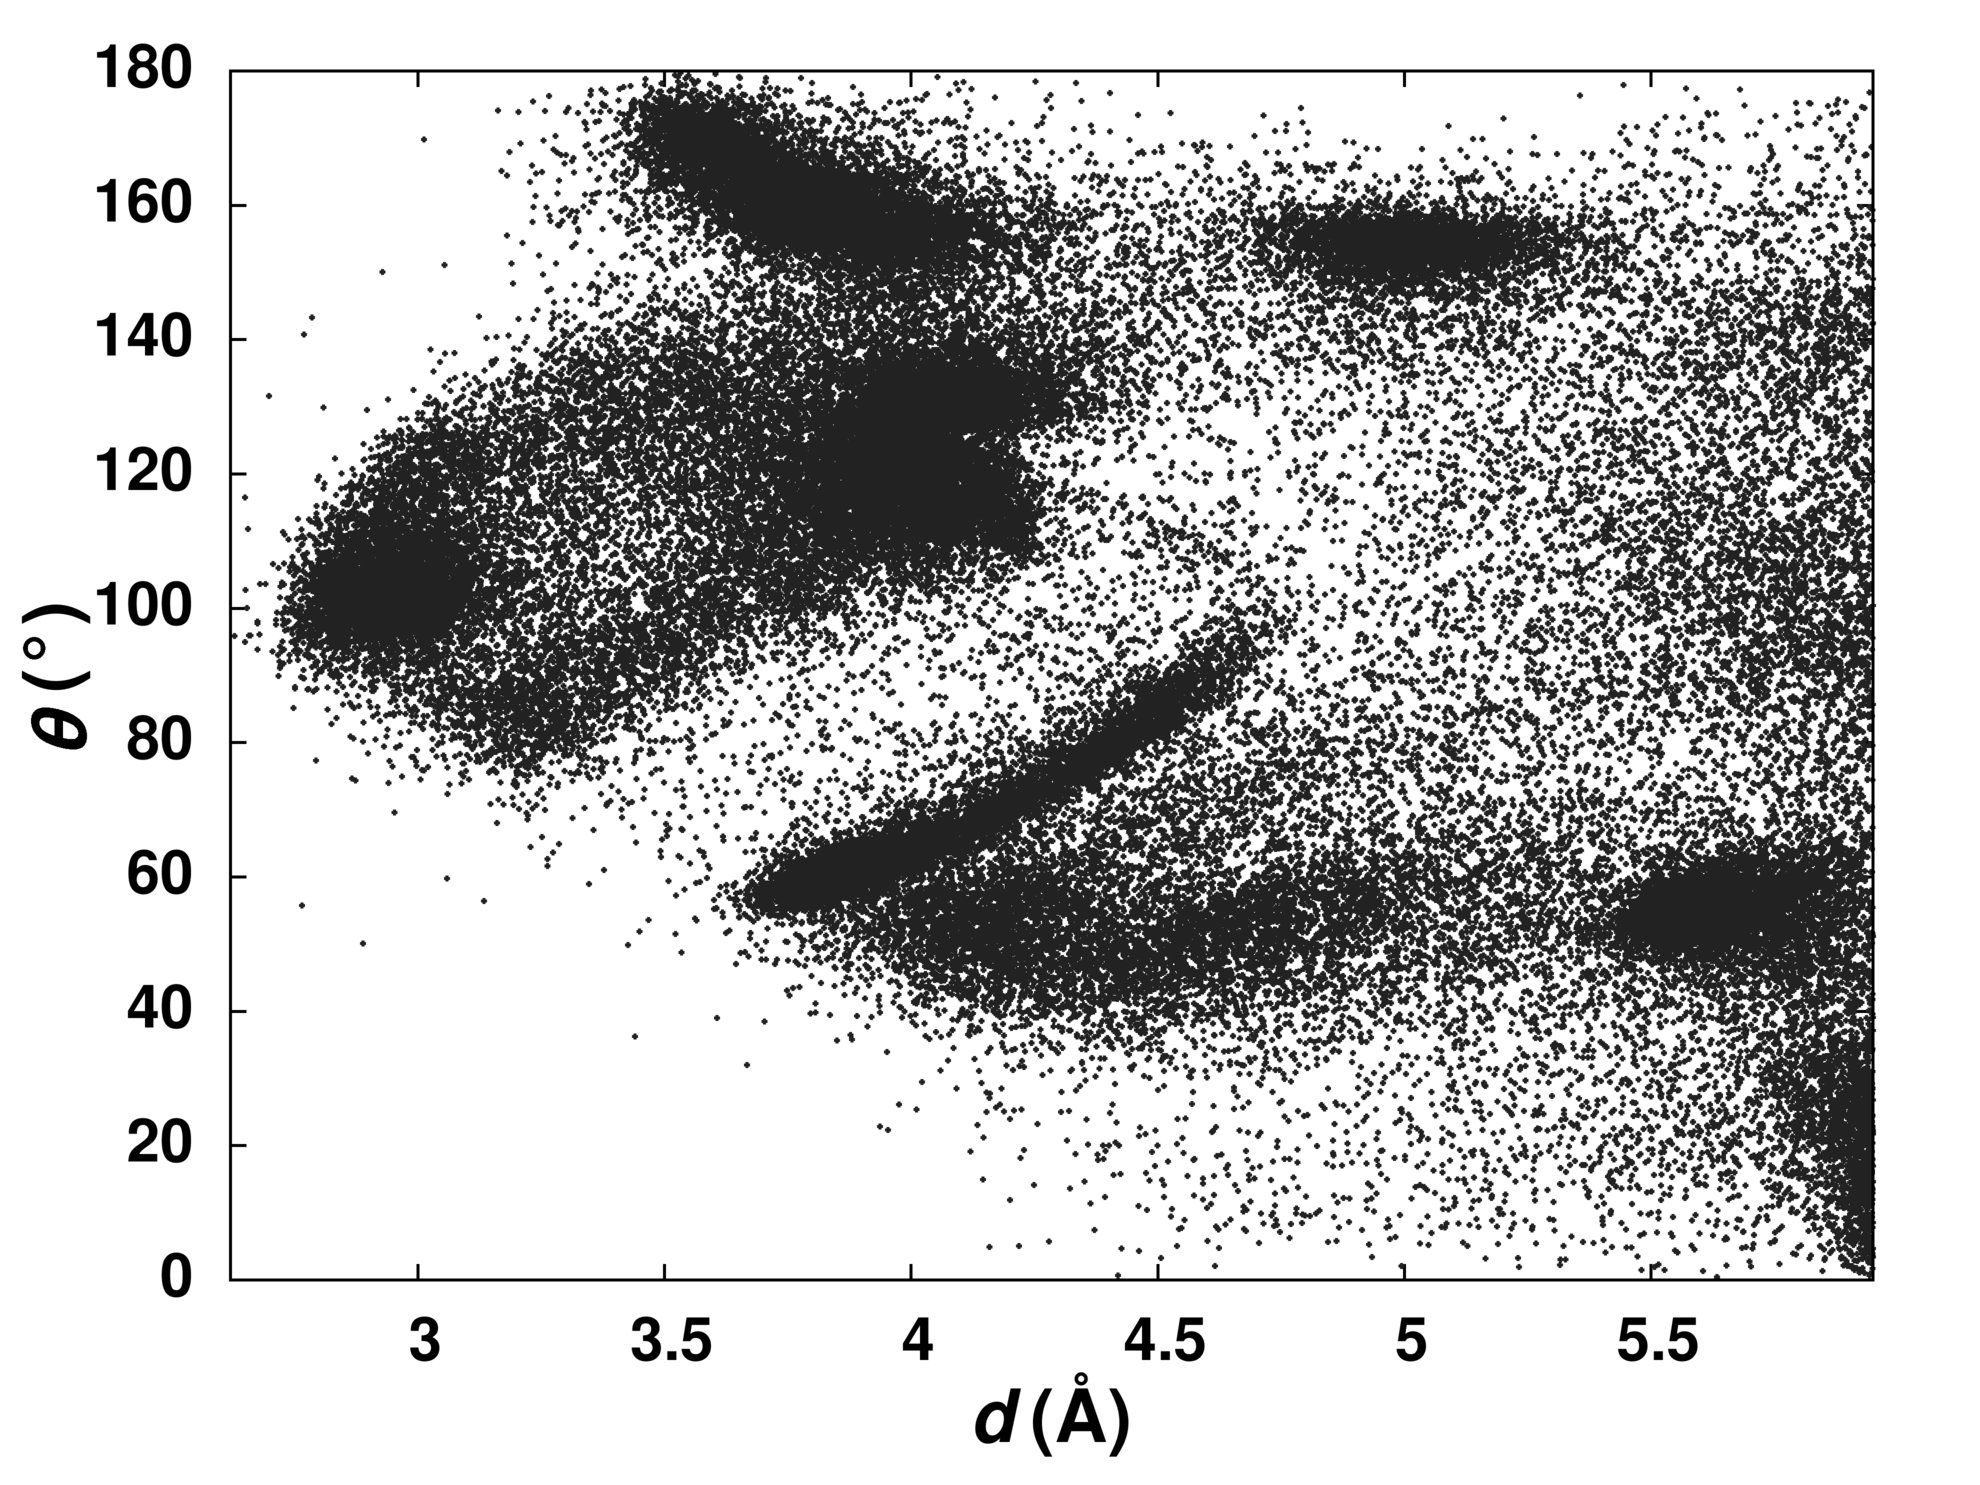
\includegraphics[width=3.5in]{figs/npistar/02.png}
\caption
      [Population of $(d,\theta)$-space by Experimental Structures.]{
  {\bf Population of $(d,\theta)$-space by Experimental Structures.}
  \\
  Plot of the distance ($d$) and angle ($\theta$) measured between each of
  the 45,792 pairs of carbonyls with a potential \npistar{} interaction. The
  relative density of points in the occupied $d$ and $\theta$ space was used
  to generate a transparency mask for Figure 9.1.
}
\end{SCfigure}

\begin{doublespace}
A set of Perl scripts was written to extract structural parameters from
the x-ray structures. For each structure in the selected set, all pairs of
residues were analyzed for the possibility of an \npistar{} interaction. Values
of $d$ and $\theta$ were calculated for each residue pair, and torsional angles
$\phi$ and $\psi$ were calculated for the `acceptor' residue of each pair.
Pairs of carbonyls with $d$ and $\theta$ values within the optimal limits for
an \npistar{} interaction were labeled as interactors (Figure 9.2). Standard
random-coil chemical shifts were subtracted from the experimental carbonyl
\cnmr{} chemical shifts for each residue.
\\\\
For all pairs of residues, a dipole-dipole potential ($V_{dd}$) was calculated
from the high-resolution x-ray structures using equation 8.1:

\begin{equation}
V_{dd} = \frac{
  \vec{\mu}_1 \cdot \vec{\mu}_2 - 3 
    (\vec{\mu}_1 \cdot \hat{r})
    (\vec{\mu}_2 \cdot \hat{r})}{
  4 \pi \epsilon_0 |\vec{r}|^3}
\end{equation}

where $\vec{\mu}_1$ and $\vec{\mu}_2$ are the two C=O bond vectors, $\vec{r}$
is the vector between the centers of the C=O bonds, and $\hat{r}$ is its unit
vector. The nominal value of 2.34 Debye was taken for the carbonyl dipole
moment. Similarly, for all residue pairs, the minimum possible hydrogen bond
length ($d_{O-H}$) was calculated from the high-resolution x-ray structures.
Hydrogen bond lengths were calculated based on the nearest non-neighboring
backbone amide hydrogen, with a maximal bonding angle of 60$^\circ$. Figure
8.3 illustrates the relationship between $V_{dd}$ and \cnmr{} chemical shifts
of all carbonyl pairs in the dataset.
\end{doublespace}

\begin{SCfigure}
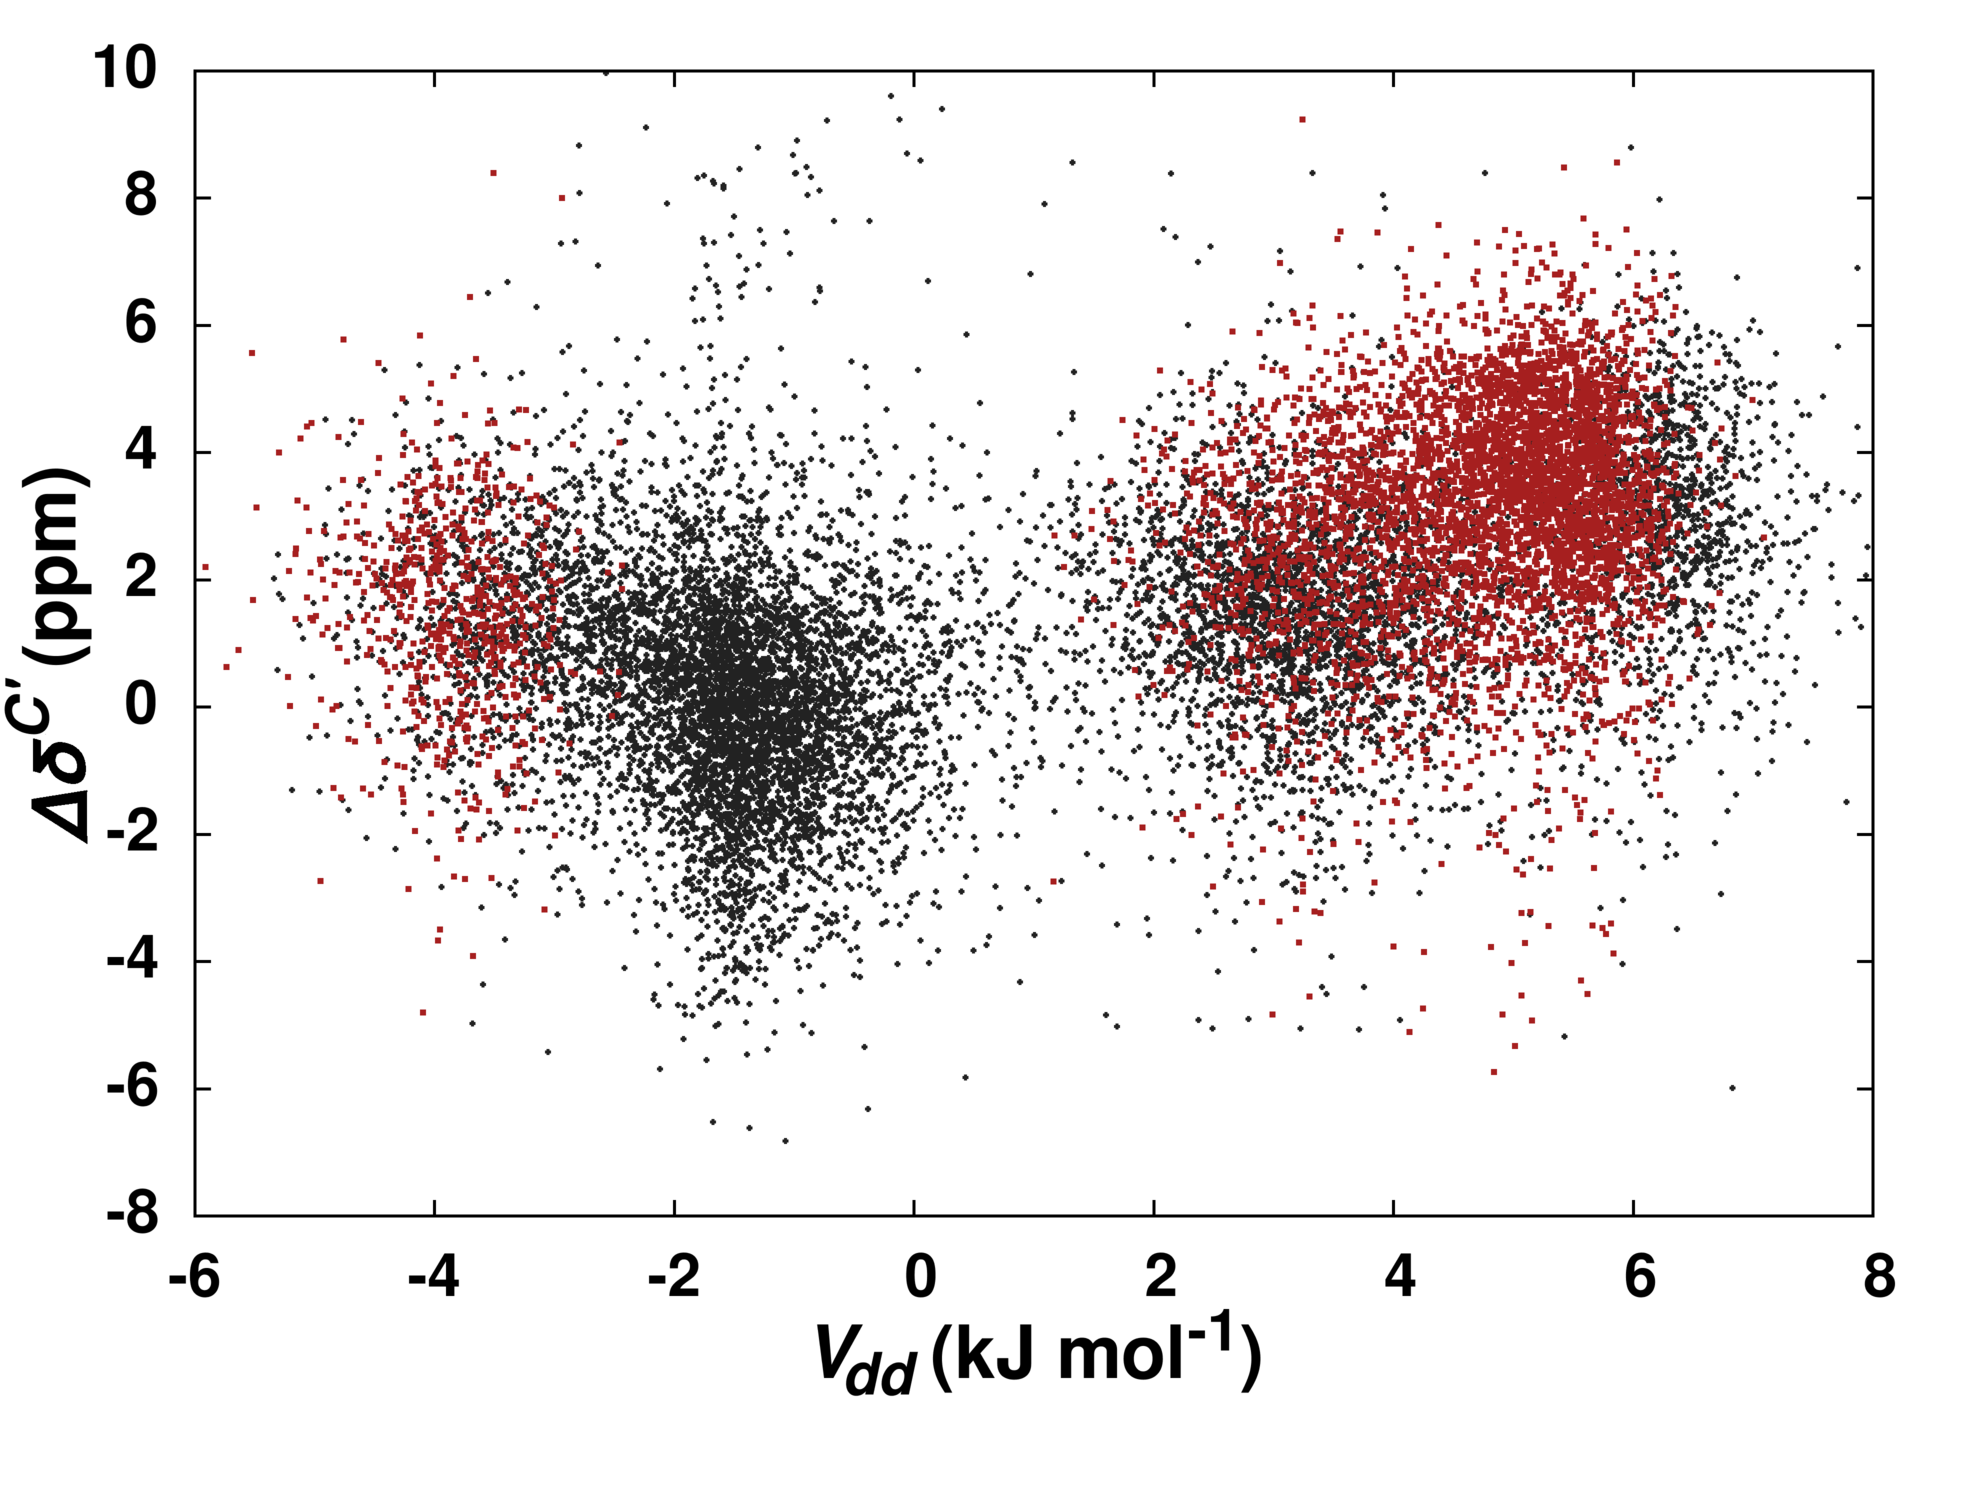
\includegraphics[width=3.5in]{figs/npistar/03.png}
\caption
      [Carbonyl \cnmr{} Chemical Shifts and Dipole-Dipole Potential.]{
  {\bf Carbonyl \cnmr{} Chemical Shifts and Dipole-Dipole Potential.}
  \\
  Carbonyl \cnmr{} chemical shift differences relative to random coil are
  plotted against calculated dipole-dipole potential ($V_{dd}$). The
  dipole-dipole potential is calculated from the high-resolution x-ray
  structure using equation 8.1. Pairs of carbonyls with $d$ and $\theta$
  values within the optimal limits for an \npistar{} interaction are colored
  red.
}
\end{SCfigure}

\subsection{Model Compound Calculations}

\begin{doublespace}
Quantum chemical calculations were performed using the program Gaussian-09
\cite{gaussian2009}. A nearly planar formamide head-to-tail dimer,
composed of a formamide monomer (molecule 1) hydrogen bonded through its C=O
group to the N-H group of a second, nearly parallel formamide (molecule 2) was
chosen to approximate the hydrogen bonding motif found in both $\alpha$-helices
and antiparallel $\beta$-sheets. The dimer was fully optimized at the
MP2/6-311++G(2d,p) level; M\"{o}ller-Plesset second order perturbation theory
(MP2) was chosen because it is superior in modeling long-range and dispersive
contributions to the electron correlation Hamiltonian. A third formamide
(molecule 3) was then added to generate the putative \npistar{} interaction
with molecule 1, imposing the following constraints:
(1) C$_3$=O$_3\cdots$C$_1$ angle fixed at 90$^\circ$, to ensure the $n_\pi$
orbital of molecule 3 points toward the carbonyl of molecule
1 (2) O$_3\cdots$C$_1$=O$_1$ constrained to a set of fixed angles $\theta$,
ranging from 70$^\circ$ to 120$^\circ$ (3) O$_3\cdots$C$_1$ constrained to
a set of fixed distances $d$, ranging from 2.9 \r{A} to 3.3 \r{A}
(5) O$_1\cdots$N$_2$ constrained to a set of fixed distances, ranging
from 2.8 \r{A} to 3.2 \r{A}, to vary the strength of the hydrogen bond. The
system of three molecules was then subjected to constrained optimization at the
same level as before. The optimized trimolecular system at an angle
$\theta = 90^\circ$ is shown in Figure 9.4. Finally, a full set of shielding
tensors was computed using standard Gauge-independent atomic orbital methods.
\end{doublespace}

\begin{SCfigure}
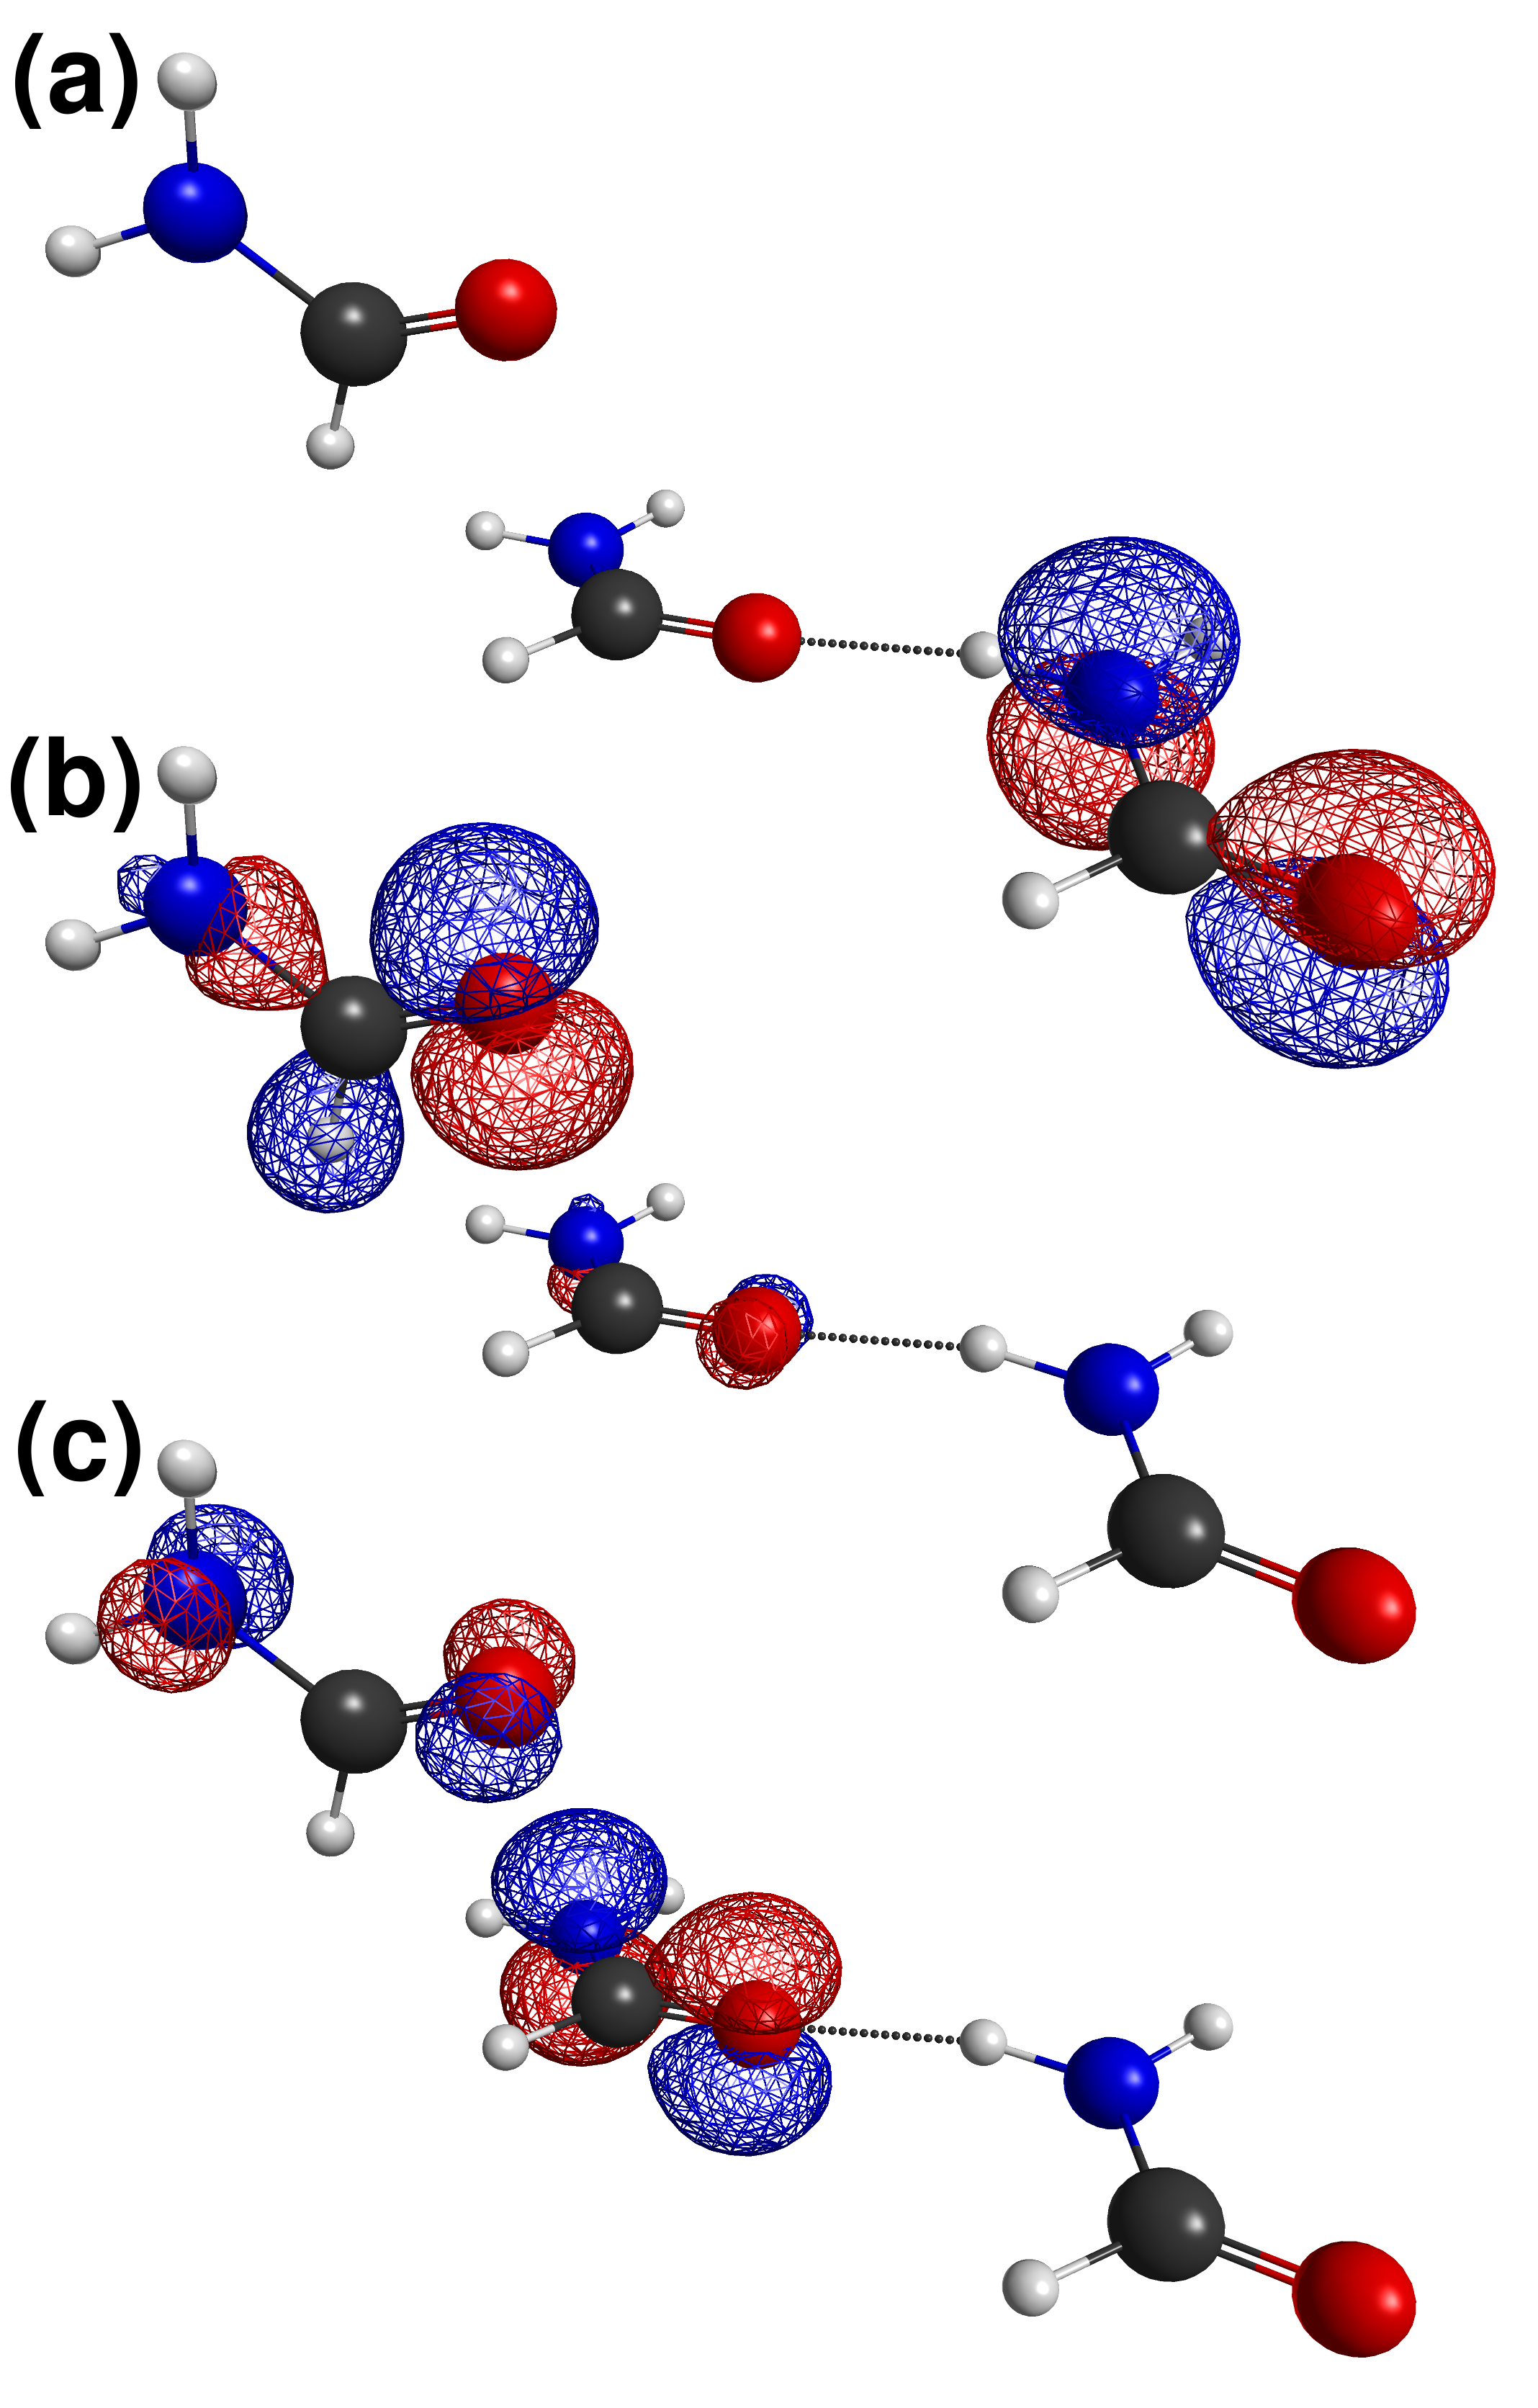
\includegraphics[width=3.5in]{figs/npistar/04.png}
\caption
      [Formamide Trimer Model.]{
  {\bf Formamide Trimer Model.}
  \\
  Molecular orbitals of ({\bf A}) the hydrogen bond donor, ({\bf B}) the
  putative \npipistar{} donor and ({\bf C}) the putative \npipistar{} acceptor,
  in the trimeric complex used in quantum chemical calculations.
}
\end{SCfigure}

\section{Results}

\begin{doublespace}
A total of 2,516,360 residue pairs from a set of 164 high-resolution
($<$ 1.6 \r{A}) x-ray crystal structures with assigned and uniformly referenced
carbonyl \cnmr{} chemical shifts were analyzed for potential \npistar{}
interactions. Setting a maximal distance of 6.0 \r{A} between the donor oxygen
and acceptor carbon yielded 45,792 potential acceptor carbonyl carbon atoms.
The carbonyl \cnmr{} chemical shift differences relative to random coil values
for each of the 45,792 potential acceptor carbonyls were plotted against the
$d$ and $\theta$ values for each carbonyl pair (Figure 9.1B). These chemical
shift differences represent the contribution from the local structural
environment, and potentially the \npistar{} interaction. The two-dimensional
contour plot indicates a maximal downfield shift of 2.9 ppm centered on the
optimal structural parameters predicted for an \npistar{} interaction.
\\\\
Of the 45,792 carbonyls, 5,378 had optimal $d$ and $\theta$ values for an
\npistar{} interaction and 40,414 were outside this optimal range. The mean
carbonyl \cnmr{} chemical shift difference for the 40,414 carbonyls labeled as
non-interactors is 0.58 $\pm$ 1.98 ppm. In contrast, the mean carbonyl \cnmr{}
chemical shift difference for the 5,378 interactors is 2.93 $\pm$ 2.41 ppm. A
Student's t-test indicates the difference of 2.35 ppm between the two means is
statistically significant at the 99.9\% confidence level. To address possible
errors introduced into the analysis by highly dynamic residues in the x-ray
structures, possible carbonyl interactors with B-factors greater than two
standard deviations above the mean were omitted from the dataset. In the
resultant set of 44,302 potential carbonyl interactors, the 2.33 ppm chemical
shift difference was statistically indistinguishable from the original
analysis. Similarly, possible interactors predicted at a 95\% confidence level
to participate in crystal-packing interfaces were also omitted from the
dataset. Again, the corresponding set of interactors yielded a chemical shift
difference of 2.33 ppm, which is still statistically significant at the 99.9\%
confidence level.
\\\\
To address the possiblity that differences between x-ray crystal structures
and NMR solution structures may lead to errors in the analysis, a replicate
analysis was performed on a set of 137 NMR solution structures corresponding
to the same set of \cnmr{} and \nnmr{} chemical shifts used previously.
Structural alignments using MAMMOTH showed a mean rmsd of 1.87 $\pm$ 0.57 \r{A}
between the pairs of x-ray and NMR structures. Of the 1,419,547 resulting
carbonyl pairs from the NMR structures, 38,534 pairs were found to be potential
interactors. Of the carbonyls in that set, 2,510 interactors were found with a
mean carbonyl \cnmr{} chemical shift difference of 2.84 $\pm$ 1.71 ppm. The
remaining 36,024 non-interactors had a mean carbonyl \cnmr{} chemical shift
difference of 1.02 $\pm$ 2.02 ppm. Again, the 1.82 ppm difference between the
two means is statistically significant at the 99.9\% confidence level, 
indicating that differences between x-ray and NMR structures cannot account
for the observed downfield \cnmr{} chemical shift.
\\\\
As predicted, a clear correlation is observed between structural regions
consistent with an optimal \npistar{} interaction and a downfield shift of the
accepting carbonyl \cnmr{} resonance. Interestingly, the potential \npistar{}
interactions were primarily observed between sequential ($|i-j|=1$) carbonyls.
Out of the 164 structures and 2,516,360 residue pairs, only four pairs of
carbonyls exhibited a through-space ($|i-j| > 5$) arrangement consistent with
an optimal \npistar{} interaction. This result implies any protein
stabilization energy obtained from the proposed \npistar{} interaction is
opportunistic, as opposed to a driving force for protein folding. Apparently,
the formation of through-space \npistar{} interactions is simply less favorable
than for other interactions, such as hydrogen bonds or salt-bridges. This also
implies that the predicted energy of 5.4 kJ/mol for an optimal \npistar{}
interaction is an over-estimate.
\\\\
In actuality, an \npistar{} interaction that imparts a stability of 5.4 kJ/mol
would likely fix adjacent pairs of carbonyl groups to preferred torsional
angles in order to maximize this interaction. Correspondingly, the existence
of these highly energetic \npistar{} interactions would likely be detrimental
to properly folding a protein structure. Folding a protein to its native fold
would require distorting the majority of carbonyl pairs away from the ideal
torsion angles for a proper \npistar{} interaction. Only ~12\% (5,378 out of
45,792) of carbonyls from the 164 x-ray structures adopted conformations with
optimal $d$ and $\theta$ values for an \npistar{} interaction. As a result,
folding every protein structure would incur an initial energetic penalty of
nearly 5.4 kJ/mol per carbonyl pair.
\end{doublespace}

\begin{SCfigure}
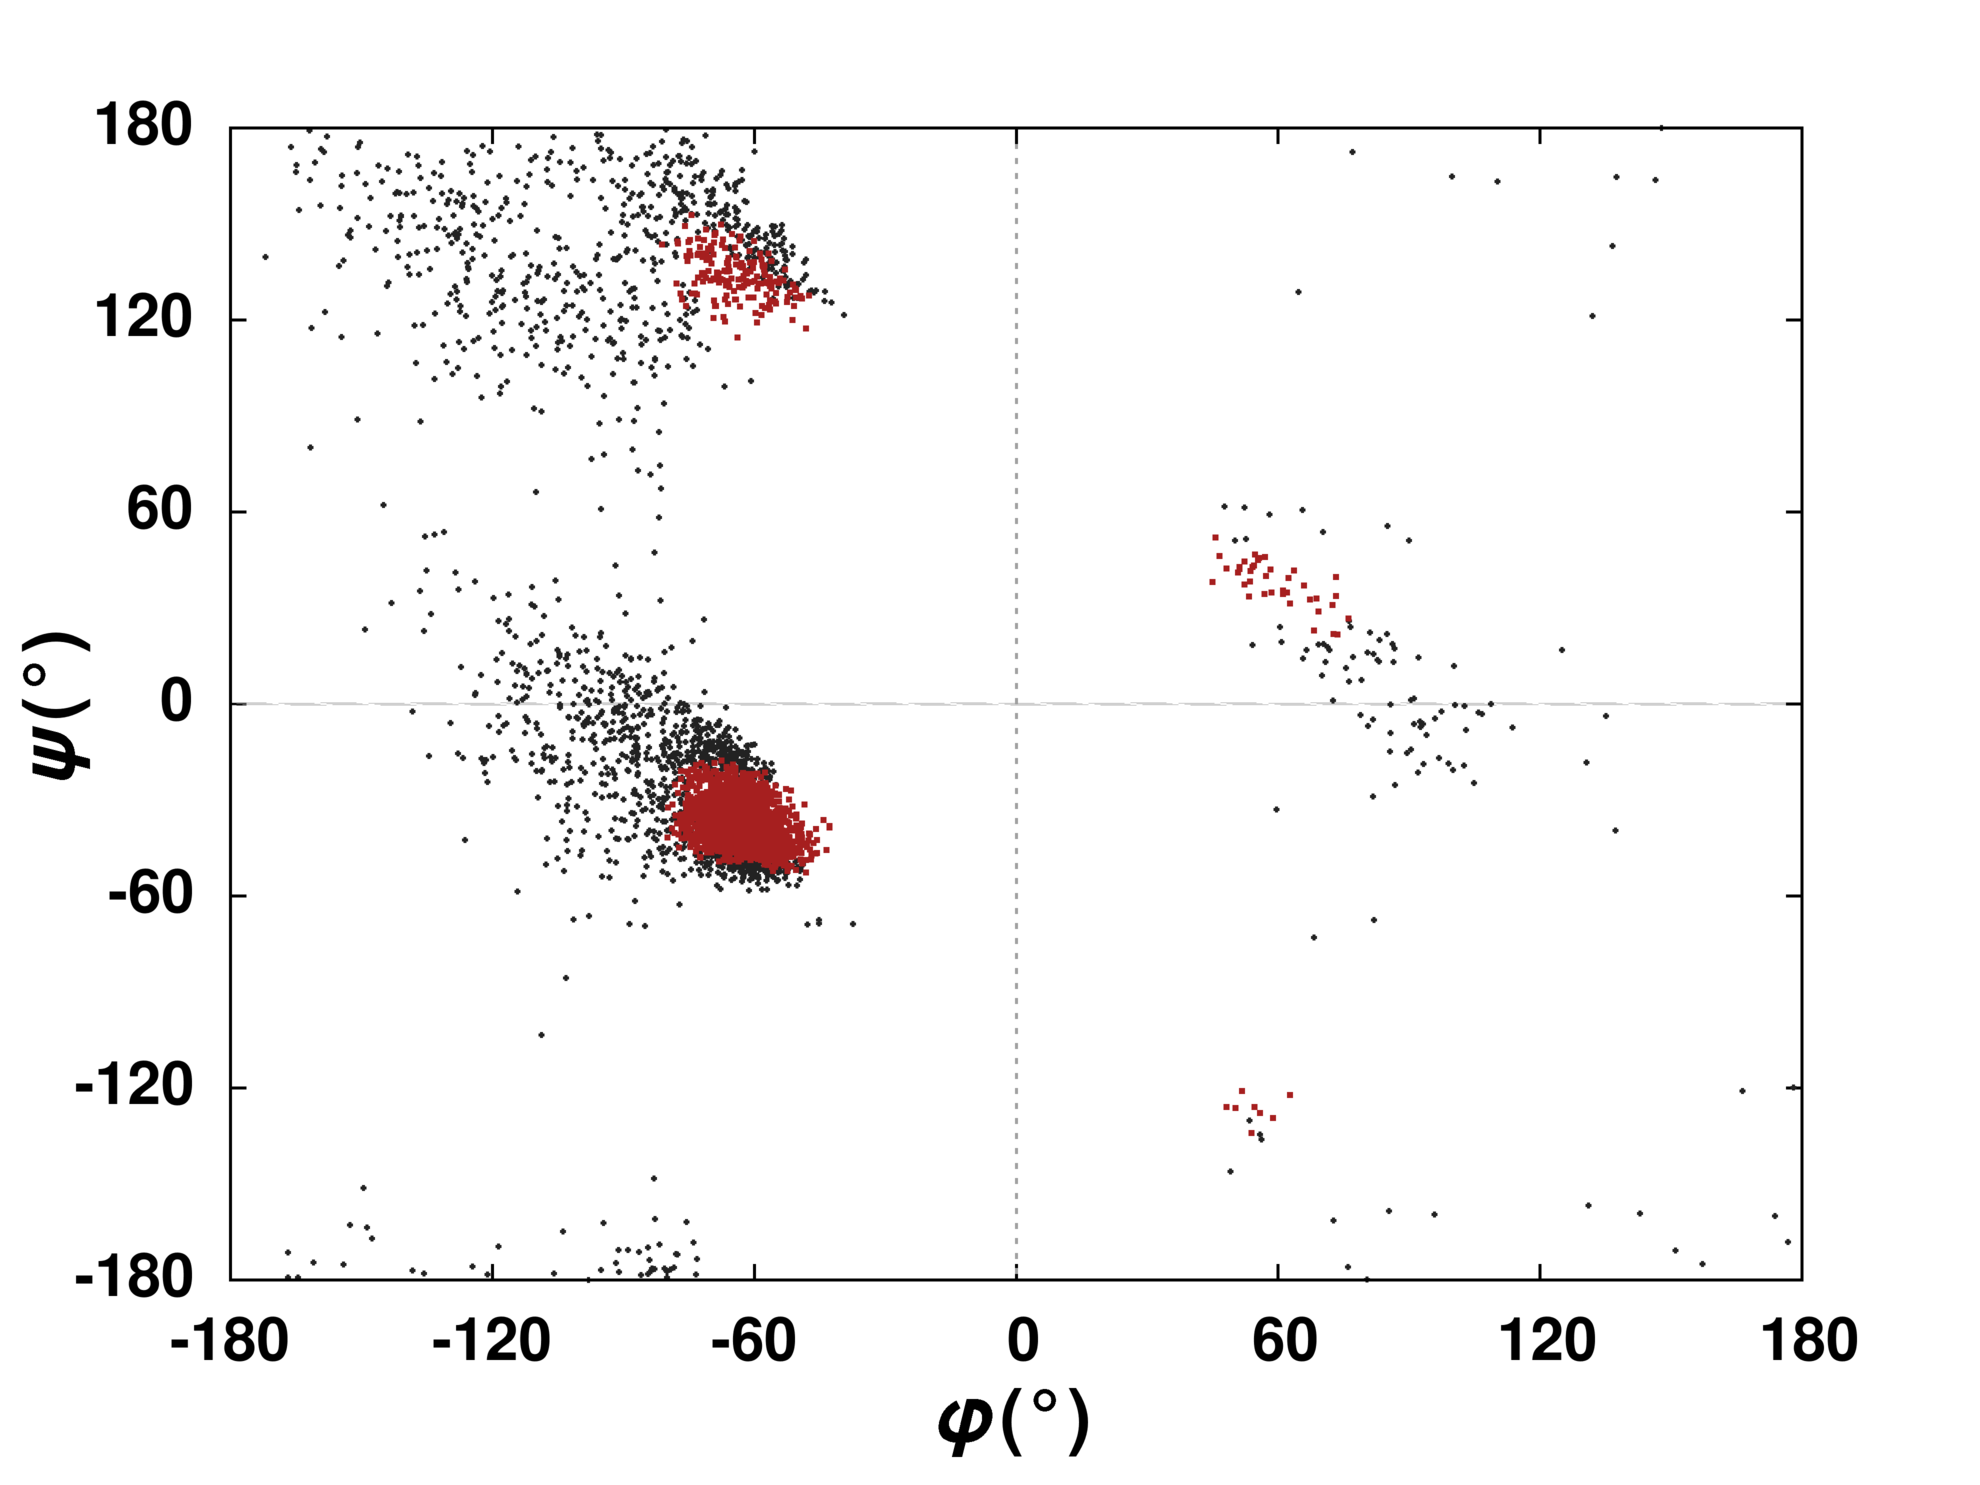
\includegraphics[width=3.5in]{figs/npistar/05.png}
\caption
      [Population of $(\phi,\psi)$-space by Experimental Structures.]{
  {\bf Population of $(\phi,\psi)$-space by Experimental Structures.}
  \\
  Ramachandran plot of carbonyls with \cnmr{} chemical shift differences
  relative to random coil that are $>$ 2.5 ppm. The acceptor carbonyls from
  each pair of carbonyls with $d$ and $\theta$ values within the optimal
  limits for an \npistar{} interaction are colored red.
}
\end{SCfigure}

\begin{doublespace}
A predominant number of the carbonyls consistent with an optimal \npistar{}
interaction and with a downfield shift of roughly 2.5 ppm fall within the
typical $\alpha$-helical region of a Ramachandran plot, where the remaining
residues are near the twisted $\beta$-sheet region (Figure 9.5). Significant
chemical shift changes for carbonyl residues within
secondary structures are well documented \cite{wang:protsci2002}.
Previous analyses of structural factors contributing to carbonyl \cnmr{}
chemical shifts have implicated hydrogen bond formation
\cite{dedios:sci1993,asakawa:jacs1992,wylie:jacs2007}
or excluded hydrogen bond formation
\cite{cisnetti:cpc2004,neal:jbnmr2003,markwick:jacs2004}, have
implicated $\phi$, $\psi$, and $\chi$ dihedral angles
\cite{neal:jbnmr2003} or have excluded secondary structure parameters
\cite{cisnetti:cpc2004,dedios:sci1993}. Thus, other factors,
such as hydrogen bonds or dipole-dipole interactions, may explain the apparent
correlation between carbonyl \cnmr{} shifts and the optimal $d$ and $\theta$
values for an \npistar{} interaction. This is probable given the association of
\npistar{} interactions with secondary structure elements. The contribution of
a dipole-dipole interaction to carbonyl \cnmr{} chemical shifts is illustrated
in Figure 9.3. The dipole-dipole potentials were calculated using the
high-resolution x-ray structures for each of the 45,792 carbonyl pairs with a
maximal distance of 6.0 \r{A} between the donor oxygen and acceptor carbon.
While there is significant scatter in the data, there is also a clear trend
between a downfield carbonyl \cnmr{} chemical shift and an increasing
dipole-dipole energy. Importantly, the cluster of acceptor carbonyls in
Figure 9.3 with the largest \cnmr{} chemical shift difference
(3.15 $\pm$ 2.44 ppm) and positive dipole-dipole potentials also conforms to
the optimal $d$ and $\theta$ values for the predicted \npistar{} interaction.
\end{doublespace}

\begin{SCfigure}
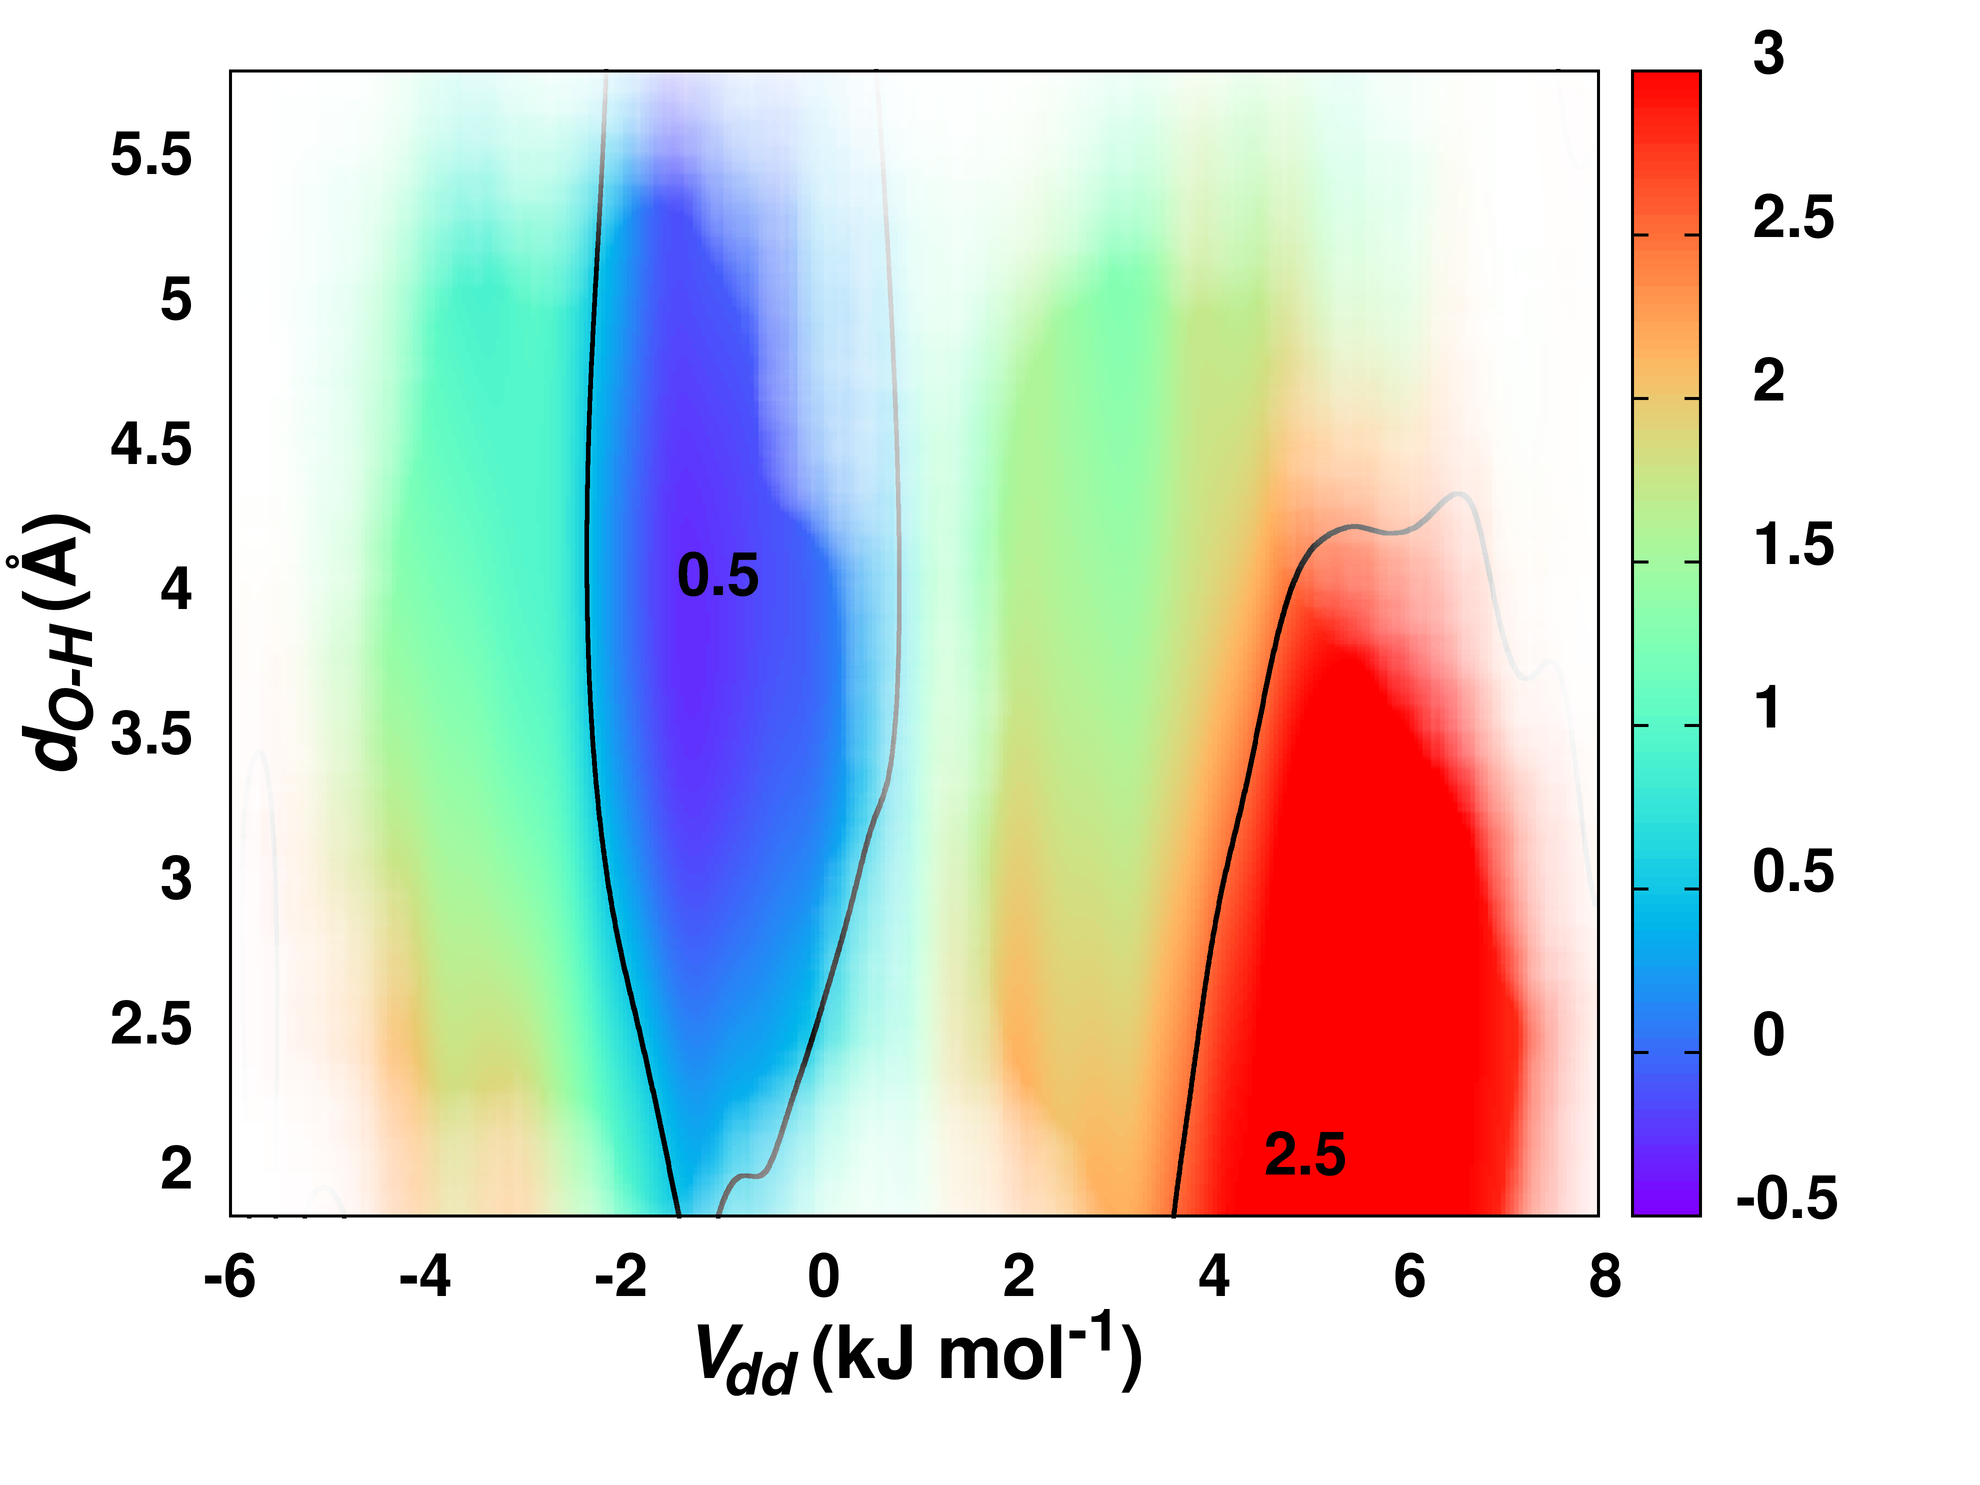
\includegraphics[width=3.5in]{figs/npistar/06.png}
\caption
      [Carbonyl \cnmr{} Chemical Shifts and Hydrogen Bonds.]{
  {\bf Carbonyl \cnmr{} Chemical Shifts and Hydrogen Bonds.}
  \\
  Contour plot of \cnmr{} carbonyl chemical shift differences as a function
  of calculated dipole-dipole potential ($V_{dd}$) and calculated hydrogen
  bond length ($d_{O-H}$).
}
\end{SCfigure}

\begin{doublespace}
The contribution of a hydrogen-bond interaction to the carbonyl \cnmr{}
chemical shift was similarly evaluated by calculating the shortest
oxygen-hydrogen distance ($d_{O-H}$) for each donor carbonyl. Again, the
distances were calculated using the high-resolution x-ray structures for each
of the 45,792 carbonyl pairs. A three-dimensional plot comparing the
dipole-dipole potentials, oxygen-hydrogen distances, and the associated
carbonyl \cnmr{} chemical shifts is very revealing. It can be clearly seen
from Figure 9.6 that any contribution from a hydrogen bond to the \cnmr{}
carbonyl chemical shift is minimal relative to the dipole-dipole contribution.
Both the $\alpha$-helical and $\beta$-sheet regions, which obviously contain
hydrogen bond interactions, have distinctly different \cnmr{} carbonyl chemical
shifts. The $\alpha$-helical region corresponds to a positive dipole-dipole
interaction, and correspondingly to a large carbonyl \cnmr{} chemical shift
difference. Conversely, the $\beta$-sheet region has a negative dipole-dipole
interaction and a near zero carbonyl \cnmr{} chemical shift difference. These
results further indicate a consistency with a dipole-dipole interaction as
opposed to the predicted \npistar{} interaction.
\\\\
It is important to note that there is a second cluster of carbonyls in Figure
9.3 with low \cnmr{} chemical shifts and negative dipole-dipole potentials that
are also consistent with the optimal $d$ and $\theta$ values for the predicted
\npistar{} interaction. A visual inspection of the x-ray structures indicates
that these carbonyl pairs are actually pointing away from each other and do not
form the configuration for an \npistar{} interaction illustrated in Figure
9.1A. Clearly, $d$ and $\theta$ values alone fail to adequately define the
optimal geometry of the dipole-dipole interaction that is apparently
responsible for the observed downfield \cnmr{} chemical shifts.
\end{doublespace}

\begin{figure}[h!]
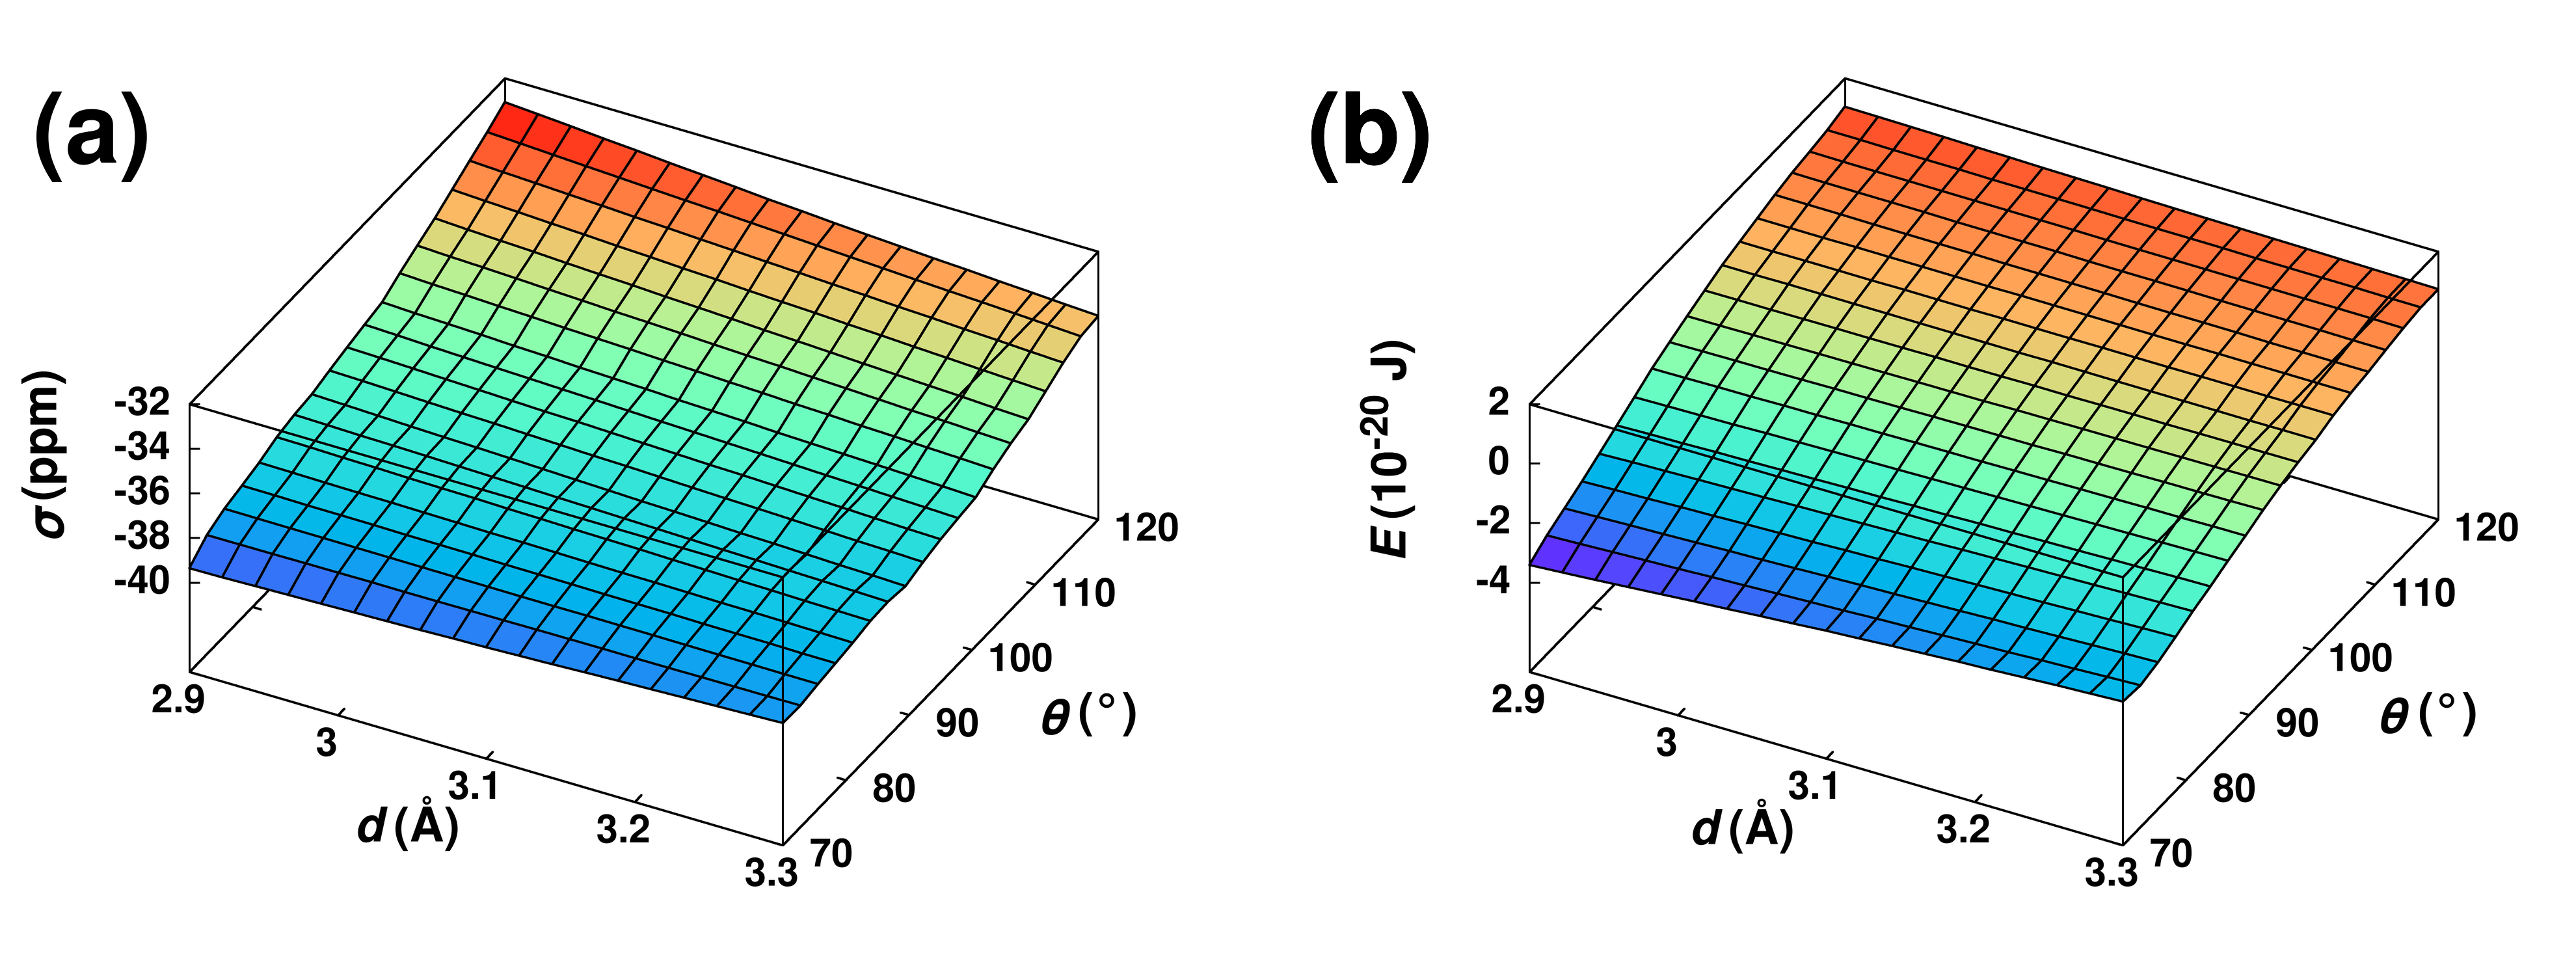
\includegraphics[width=6.5in]{figs/npistar/07.png}
\caption
      [Summary of Quantum Chemical Calculations.]{
  {\bf Summary of Quantum Chemical Calculations.}
  \\
  Plot of calculated ({\bf A}) carbonyl \cnmr{} chemical shielding ($\sigma$)
  and ({\bf B}) dipole-dipole interaction energy ($E$) as a function of the
  distance between donor oxygen and acceptor carbon ($d$) and the angle
  between carbonyl groups ($\theta$).
}
\end{figure}

\begin{doublespace}
To further examine the origin of these effects, quantum chemical calculations
were conducted on a model system, a formamide trimer in which molecules 2 and 3
form an approximately planar, head-to-tail hydrogen bonded dimer, and molecule
3 acts as a putative \npistar{} donor, with the $n_\pi$ `donor' oxygen fixed at
a distance $d$ which ranges from 2.9 \r{A} and 3.3 \r{A} from the carbonyl
carbon of molecule 2, with the O$_3\cdots$C$_2$ vector also fixed at angles
$\theta$ from 70$^\circ$ to 120$^\circ$ from the C$_2$=O$_2$ vector. To avoid
problems with the use of density functional theory to model virtual
orbitals, M\"{o}ller-Plesset second order perturbation theory (MP2) was
instead used, with a substantially larger basis set than in the previous work.
The geometry and relevant Hartree-Fock orbitals of the complex used is shown
in Figure 9.4, for $d$ = 2.9 \r{A} and $\theta = 100^\circ$. The computed
chemical shielding is shown in Figure 9.7A as a function of $d$ and $\theta$.
The shielding decreases monotonically with $\theta$, but, in contrast, the
slope of the shielding surface with respect to $d$ changes sign between
$\theta = 70^\circ$ and $\theta = 120^\circ$. This shielding surface does not
have the geometry expected if the chemical shielding dependencies on $\theta$
and $d$ were dominated by an \npipistar{} interaction, where shielding should
be maximal at $\theta$ slightly larger than 90$^\circ$ and $d$ = 2.9 \r{A},
decreasing rapidly with increasing values of $d$.
\\\\
However, the shielding surface does show a remarkable similarity to the
dipole-dipole energy between the putative donor and acceptor, as shown in
Figure 9.7B. This energy was computed using a very simple model assuming the
electric dipole vector lies along the carbonyl bond for both molecules and has
a value of 2.34 D or $7.81 \times 10^{-30}$ C$\cdot$m. As can be seen, the
dipole energy closely parallels the chemical shielding surface, monotonically
increasing with $\theta$ and inverting its slope with respect to $d$ as
$\theta$ increases. This indicates the major influence on the carbonyl \cnmr{}
chemical shielding is not an \npipistar{} interaction but rather the
electrostatic field from the neighboring carbonyl dipole. The correspondence
is not, however, exact: the chemical shielding surface shows a small negative
inflection around $\theta = 90^\circ$, which is actually slightly reversed in
the dipolar energy plot.
\end{doublespace}

\begin{figure}[h!]
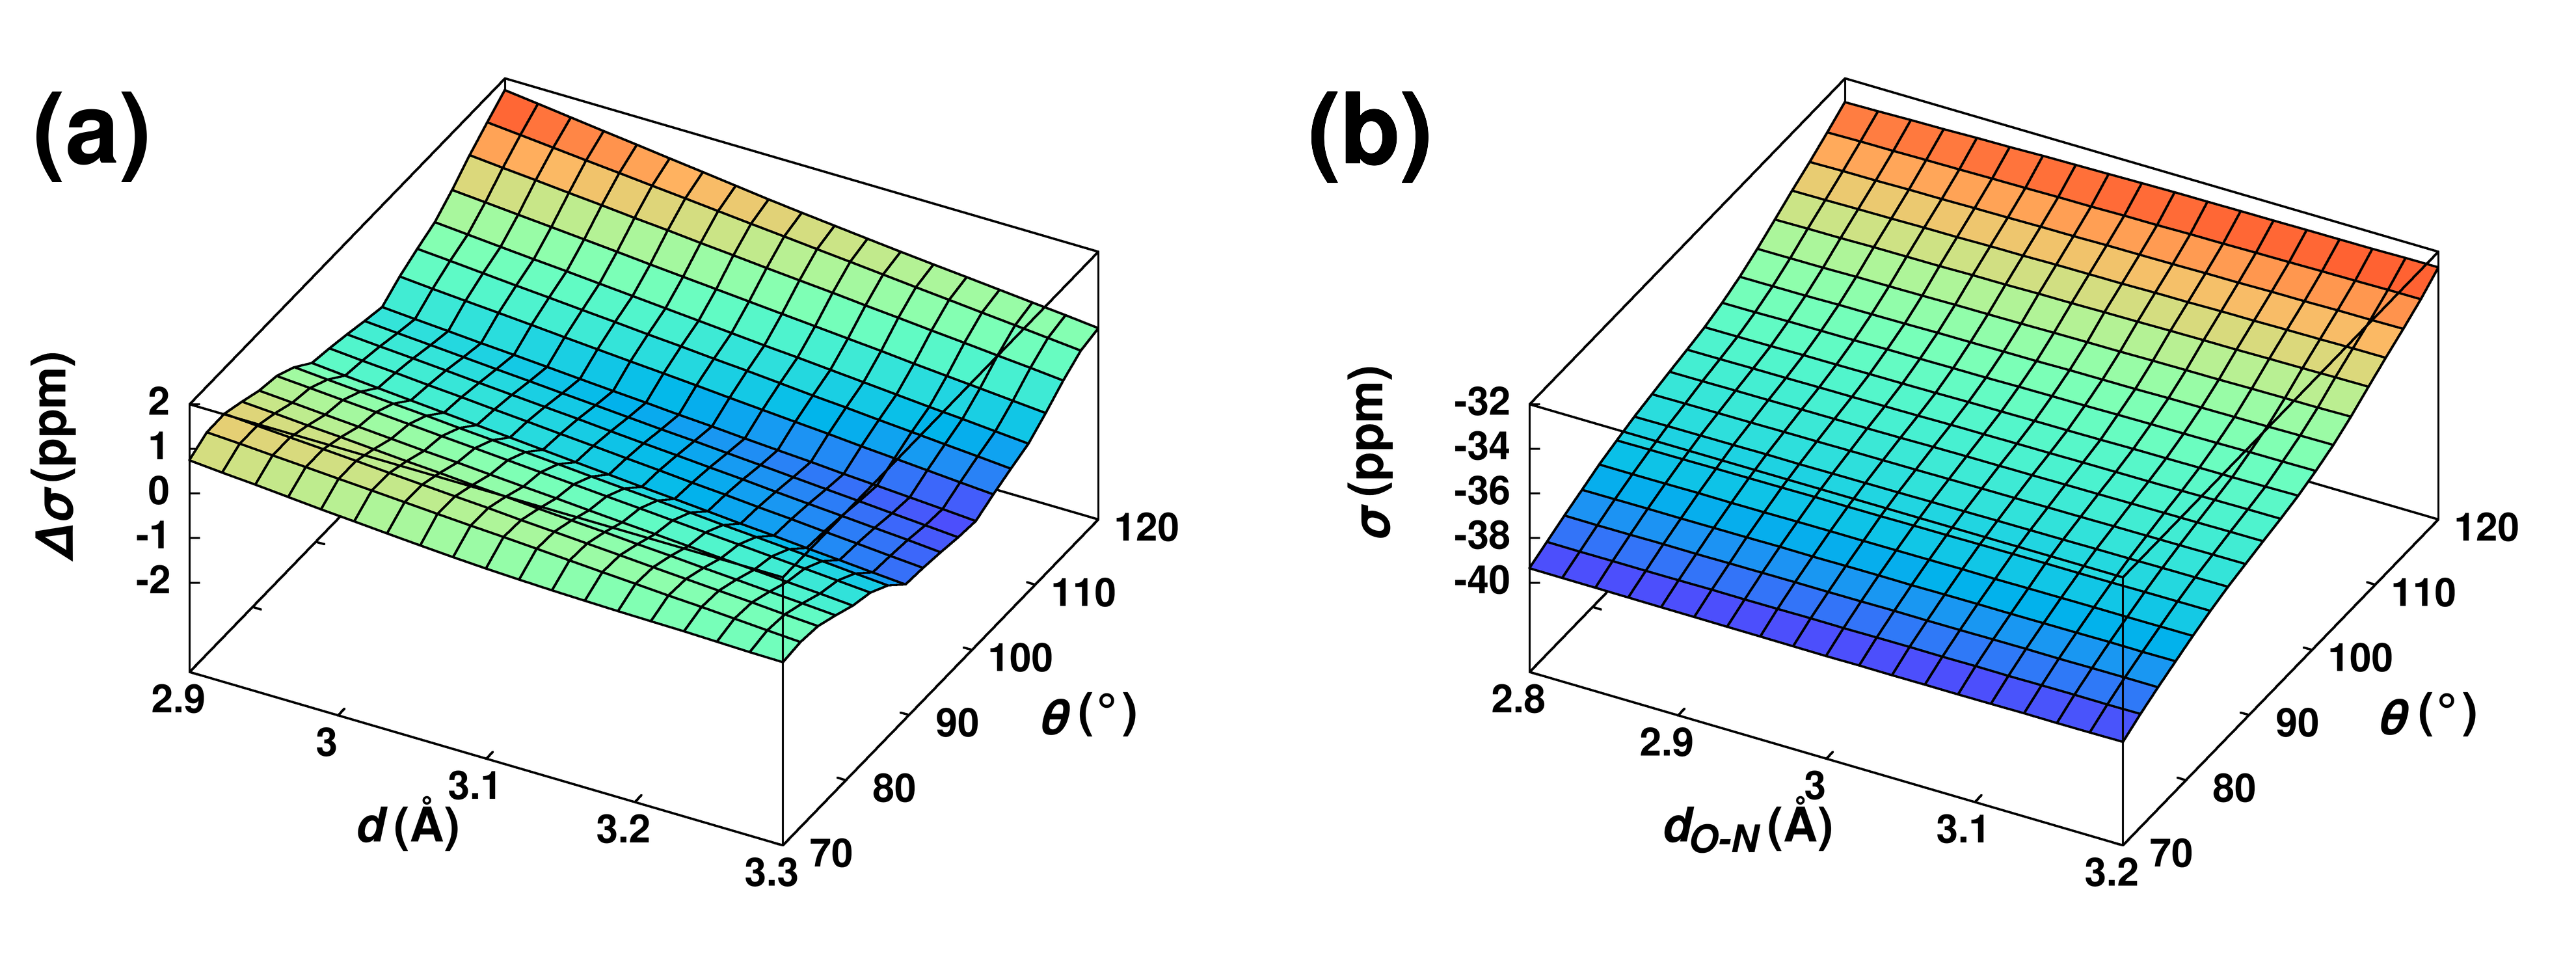
\includegraphics[width=6.5in]{figs/npistar/08.png}
\caption
      [Supplemental Quantum Chemical Results.]{
  {\bf Supplemental Quantum Chemical Results.}
  \\
  ({\bf A}) Plot of the residuals for the fit of the chemical shielding
  surface to a function proportional to the dipole-dipole energy.
  ({\bf B}) Summary of the quantum chemical calculations of the hydrogen
  bond contribution to the dipole-dipole interaction; plot of carbonyl \cnmr{}
  chemical shielding ($\sigma$) as a function of the hydrogen bond angle
  ($\theta$) and distance ($d_{O-N}$).
}
\end{figure}

\begin{doublespace}
In order to examine whether an \npipistar{} interaction might be responsible
for this inflection, the chemical shielding surface was fit to a function
proportional to the dipolar energy, under the assumption the dipole moment
vector lies along the C=O bond direction, and the best fit subtracted from the
chemical shielding surface (Figure 9.8A). The residual shows a
minimum at $\theta \sim 95^\circ$, as would be expected for an \npipistar{}
interaction, but the dip does not appear to decrease rapidly as $d$ increases,
as an orbital overlap term would. In fact, the residual is slightly larger at
$d$ = 3.3 \r{A} than at 2.9 \r{A} (1.3 ppm vs. 1.1 ppm).
\\\\
From the fit of the shielding surface to the estimated dipole interaction
energy, with the assumption the magnitude of the electric dipole moment is
that of a formamide monomer (3.7 D), a dependence of chemical shielding on
field of $-190$ ppm/a.u. was obtained (1 atomic unit (a.u.) of electric field
equals $5.142\times10^{11}$ V/m). Direct calculations of the dependence of the
shielding of an isolated formamide on an external applied field along the C=O
bond direction gave a value of $-150$ ppm/a.u. However, it is highly likely
that this estimation of the dipole-dipole interaction for two amides is low.
Firstly, higher electric multipole terms were neglected in the calculation,
and these are likely to be substantial for a moiety as asymmetric as a peptide
linkage, at these close proximities. Second, the interaction of the dipoles
is likely to be enhanced by the highly polarizable hydrogen bond, which is
necessarily omitted in the monomer model. Agreement of the model with direct
estimates of the effect of electric field on shielding is therefore rather
good.
\\\\
The dependence of chemical shielding on hydrogen bonding strength for all
combinations of $d$ and $\theta$ was examined as a function of the hydrogen
bond distance $d_{O-N}$ (see Supplemental Figure 9.8B). In accordance with the
results of Wishart and others
\cite{cisnetti:cpc2004,neal:jbnmr2003,markwick:jacs2004}, and contrary
to initial na\"{i}ve expectations, the effect was very small and independent of
the position of the putative \npipistar{} donor carbonyl.
\end{doublespace}

\begin{figure}[h!]
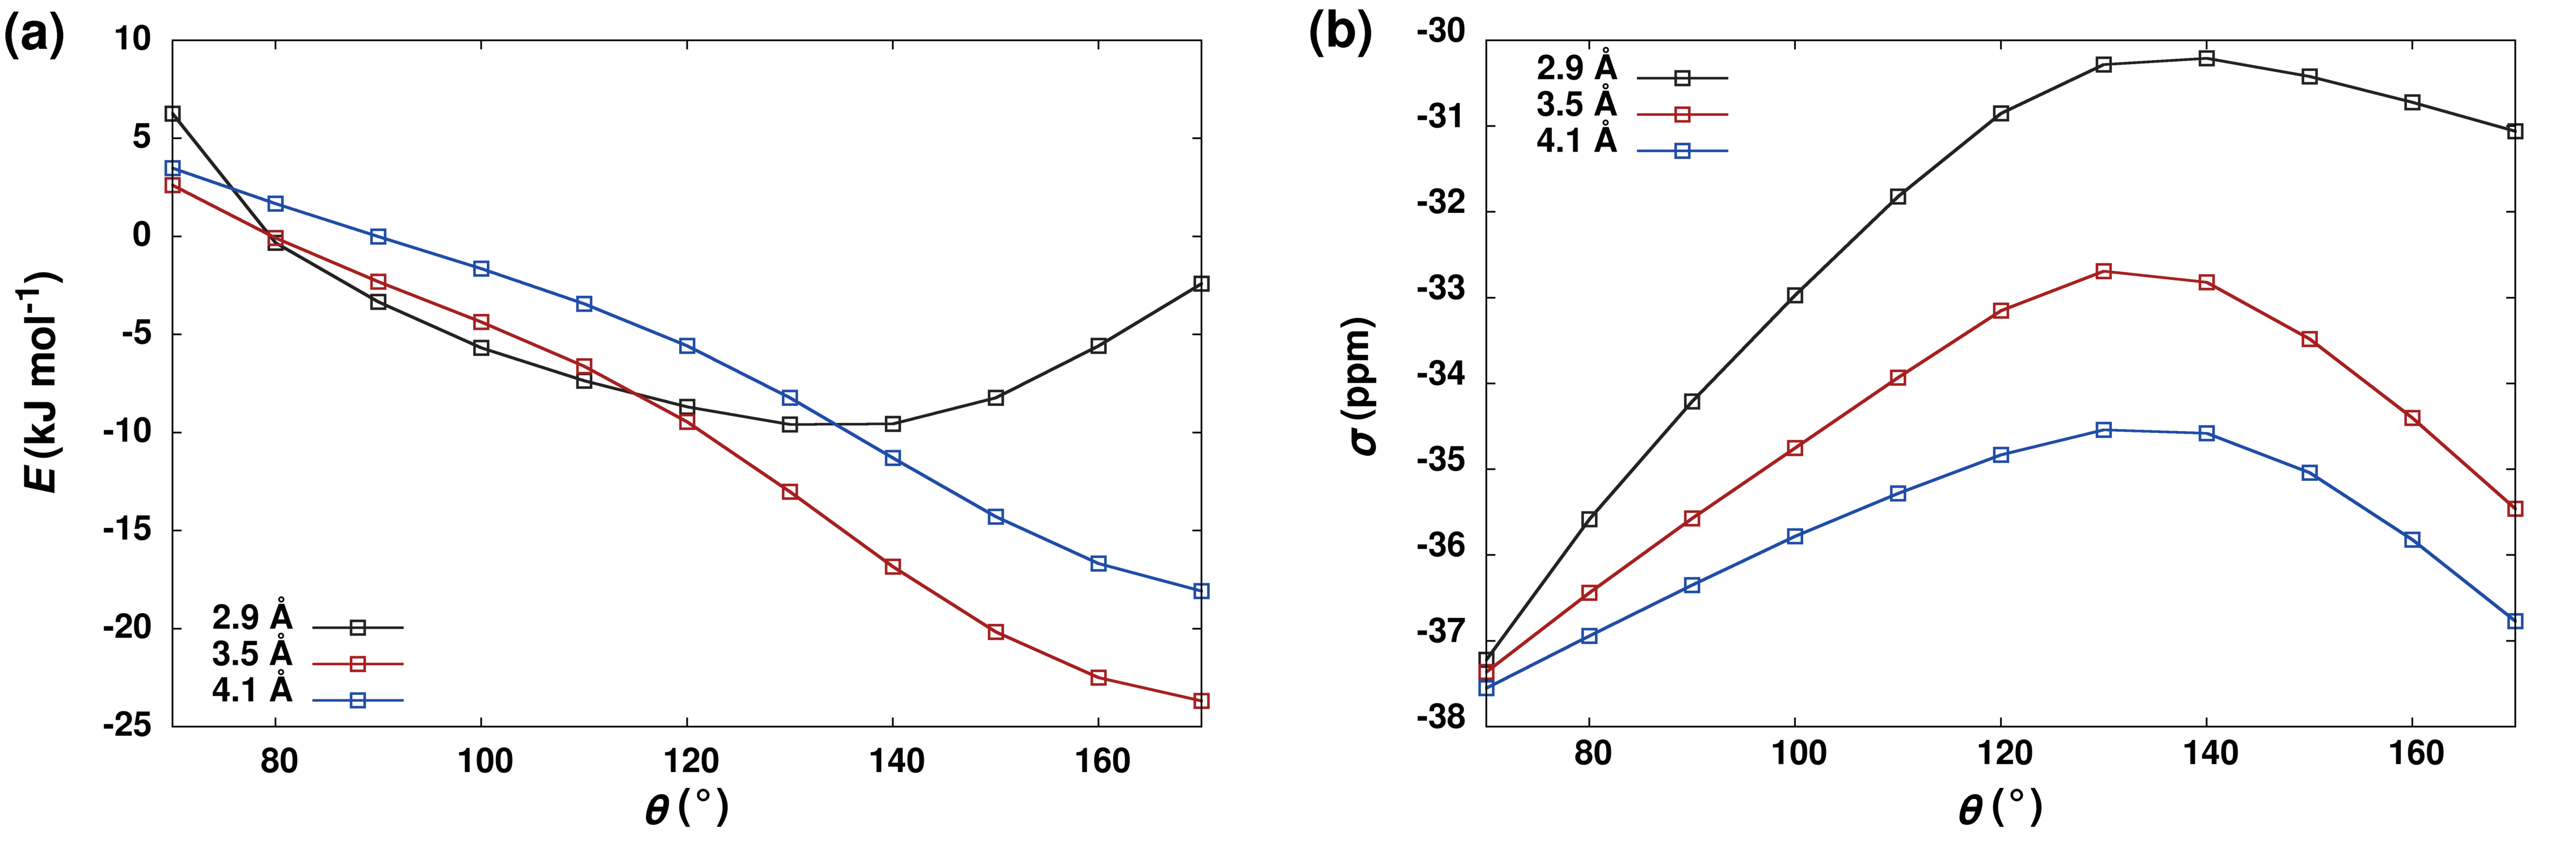
\includegraphics[width=6.5in]{figs/npistar/09.png}
\caption
   [Summary of Quantum Chemical Calculations for `End-On' Dipole Interaction.]
  {{\bf
    Summary of Quantum Chemical Calculations for `End-On' Dipole Interaction.
  }
  \\
  Plots of ({\bf A}) interaction energy and ({\bf B}) carbonyl \cnmr{} chemical
  shielding ($\sigma$) as a function of the angle between the carbonyls
  ($\theta$) for three different distances ($d$) between the donor oxygen
  and acceptor carbon.
}
\end{figure}

\begin{doublespace}
For the sake of completeness, the effect of an `end-on' carbonyl-carbonyl
interaction was examined, using a dimeric cluster in which the `donor' carbonyl
bond was parallel to the `donor' oxygen-`acceptor' carbon vector, resulting in
a possible \nspistar{} interaction. As can be seen in Figure 9.9, for values of
$d$ ranging from 2.9 \r{A} to 4.1 \r{A}, the chemical shielding also follows
the negative of the dipolar interaction energy over the range
$70^\circ < \theta < 120^\circ$, with little evidence of any effect of orbital
overlap on chemical shielding.
\\\\
One other outcome of the calculations is of possible note. While there was
little discernible effect of the proposed \nspistar{} or \npipistar{}
interactions on the shielding of the carbonyl carbon or the length of the
carbonyl bond, substantial pyramidalization of the amide nitrogen was observed
at low values of $d$ and values of $\theta$ close to 90$^\circ$. This would
indicate that the primary effect of the `donor' carbonyl might not be on the
carbonyl $\pi$ bond \emph{per se}, but on its delocalization over the entire
amide group. There was also a substantial lengthening of the carbon-nitrogen
bond -- consistent with a reduced bond order -- accompanied by substantial
changes in the computed \nnmr{} chemical shielding. Thus, while no evidence
was found of effects from \nspistar{} interactions on the \cnmr{} NMR
spectroscopy or the energetics of the system, such interactions might be
detectable in \nnmr{} chemical shifts. Unfortunately, \nnmr{} shifts are known
to be much more dispersed than carbonyl \cnmr{} shifts and are susceptible to
a wide range of influences, so disentangling the interaction in real proteins
might be a Herculean task.
\end{doublespace}

\section{Discussion and Conclusions}

\begin{doublespace}
When the molecular orbitals for the trimeric complex are examined in detail, 
the above results become clear. It is in fact misleading to think of amide 
groups as being dominated by the carbonyl $\pi$ bond. The highest occupied
molecular orbital (HOMO) of the formamide trimer in fact consists almost
entirely of $p_z$ orbitals on the N and O, with wavefunctions of opposite sign.
This is depicted in Figure 9.4A for the Hartree-Fock HOMO of the hydrogen bond
donor (energy = $-0.377$ Ha). The orbital is slightly bonding with respect to
the carbonyl, but the carbonyl carbon overall has very little contribution to
the molecular orbital. The equivalent orbital of the putative acceptor
(Figure 9.4B) has somewhat lower energy ($-0.438$ Ha) but shows remarkably
little mixing with other molecular orbitals, and in particular little mixing
with the $n_\pi$ orbital of the putative \npipistar{} donor (Figure 9.4C). That
orbital has in fact a very similar energy ($-0.465$ Ha), and at other
geometries -- specifically lower values of $\theta$, mixes with the HOMO of
the acceptor. The reason for this is quite simple: because the HOMO has only a
very small contribution for carbonyl carbon orbitals, bringing the $n_\pi$
orbital closer to it has very little effect. The mixing that is present at
smaller values of $\theta$ in fact seems to be partly responsible for the
increased pyramidalization of the nitrogen of the acceptor at those
orientations. We see no evidence of any orbital mixing that could be attributed
to \npipistar{} interactions. Given the weakness of the mixing with orbitals
that are very close in energy to $n_\pi$ it is implausible that substantial
mixing would be observed with an orbital almost a Hartree higher in energy.
\\\\
In conclusion, quantum chemical calculations, experimental carbonyl \cnmr{}
chemical shifts and structural data indicate that a simple electrostatic
dipole-dipole interaction explains the large downfield carbonyl \cnmr{}
chemical shift in an $\alpha$-helix. There is no evidence for a significant
contribution from an \npistar{} interaction to the carbonyl bond. The single
indication of \npistar{} interactions seems to be a substantial lengthening of
the carbon-nitrogen bond and pyramidalization of the nitrogen at $\theta$
angles favorable for these interactions. In fact, such pyramidalization seems
to be a logical consequence of the electronic structure of amides, whose $\pi$
orbitals are delocalized over the whole system.
\end{doublespace}

\bibliographystyle{abbrv}
\bibliography{bworley}

